\باب{امالی مشین}
گزشتہ برسوں میں \اصطلاح{قوی الیکٹرانکس}\فرہنگ{قوی الیکٹرانکس}\حاشیہب{power electronics} کی میدان میں بہت ترقی ہوئی۔اس کا ایک نتیجہ یہ نکلا کہ امالی موٹروں کی رفتار پر قابو رکھنا ممکن ہوا اور یوں ان موٹروں نے کارخانوں میں یک سمتی رو موٹروں کی جگہ لینی شروع کی۔یہاں یہ بتلاتا چلوں کہ اس سے پہلے جہاں بھی موٹر کی رفتار اہمیت رکھتی وہاں یک سمتی رو موٹر ہی استعمال ہوتی جن کی رفتار پر قابو رکھنا نہایت آسان ہوتا ہے۔پچاس سال پہلے ترقی یافتہ ممالک میں یک سمتی سے امالی آلوں کی جانب تبدیلی شروع تھی۔ آج میں یہی تبدیلی پاکستان میں دیکھ رہا ہوں۔ امالی موٹروں کی مضبوطی اور دیرپا کام کرنے کی صلاحیت مثالی ہے۔ قوی الیکٹرانکس نے ان کی بے قابو رفتار کو قابو کر کے انہیں بلا مقابلہ بنا دیا۔

امالی موٹر ٹرانسفارمر کی ایک اور شکل ہے یا یوں کہنا بہتر ہو گا کہ یہ ایک ایسا ٹرانسفارمر ہے جس میں ثانوی لچھا حرکت بھی کرتا ہے۔یوں امالی موٹر کے ساکن لچھے ٹرانسفارمر کے ابتدائی لچھے اور موٹر کے گھومتے لچھے ٹرانسفارمر کے ثانوی لچھوں کی جگہ ہوتے ہیں۔موٹر کے ساکن لچھوں کو بیرونی برقی طاقت دی جاتی ہے جبکہ اس کے گھومتے لچھوں میں خلاء میں گھومتے مقناطیسی موج سے پیدا امالی برقی دباؤ ہی کام آتی ہے۔اسی سے اس کا نام امالی موٹر نکلا ہے۔

 اس باب کا مقصد امالی موٹر کی مساوی دور یعنی \اصطلاح{ریاضی نمونہ}\فرہنگ{ریاضی نمونہ}\حاشیہب{mathematical model}\فرہنگ{model} بنا کر اس کی خصوصیات پر غور کرنا ہے۔ہم دیکھیں گے کہ ان کا مساوی دور ٹرانسفارمر کے مساوی دور کی طرح کا ہے۔

یہاں بھی ہم تصور کرتے ہیں کہ موٹر دو قطب اور تین مرحلہ ہے اور اس کے لچھے ستارہ نما جڑے ہیں۔اس طرح یک مرحلہ لچھوں میں برقی رو، تار کی برقی رو ہی ہو گی اور ان پر لاگو برقی دباؤ، یک مرحلہ برقی دباؤ ہو گی۔ایسا کرنے سے مسئلہ پر غور کرنا آسان ہو جاتا ہے جبکہ نتیجہ کسی بھی موٹر کے لئے درست ہوتا ہے۔

\حصہ{ساکن لچھوں کی گھومتی مقناطیسی موج}
امالی مشین کے ساکن لچھے بالکل معاصر مشین کے ساکن لچھوں کی طرح ہوتے ہیں۔مزید یہ کہ اس کے گھومتے حصے کے اتنے ہی قطب ہوتے ہیں جتنے اس کے ساکن لچھوں کے ہوتے ہیں ۔اگر ان ساکن لچھوں کو متوازن تین مرحلہ برقی رو سے ہیجان کیا جائے تو یہ ایک گھومتے مقناطیسی دباؤ کی موج کو جنم دیں گے جسے مساوات  \حوالہ{مساوات_تبادلہ_گھومتا_موج} میں دکھایا گیا ہے۔مساوات \حوالہ{مساوات_گھومتے_مشین_برقی_میکانی_رفتار_تعلق}  اس موج کی معاصر رفتار دیتی ہے۔یہ دونوں مساوات یہاں یاد دھیانی کے لئے دوبارہ دیئے جاتے ہیں۔یہاں ساکن لچھوں میں برقی رو کی تعدد \عددیء{\omega_e} لکھی گئی ہے اور \عددیء{\theta_0} کو صفر لیا گیا ہے۔
\begin{gather}
\begin{aligned}\label{مساوات_امالی_گھومتا_مقناطیسی_دباؤ_الف}
\tau_s^+ (\theta,t)&=\frac{3 \tau_0}{2} \cos (\theta-\omega_ t)\\
f_m&=\frac{2}{P} f_e
\end{aligned}
\end{gather}

\حصہ{مشین کی سرکنے اور گھومتی موجوں پر تبصرہ}
ہم دو قطب کے مشین پر غور کر رہے ہیں۔\عددیء{P} قطب کا تذکرہ بھی بالکل اسی طرح ہے۔ساکن لچھوں میں تین مرحلہ برقی رو کی تعدد \عددیء{f_e} ہے۔مساوات \حوالہ{مساوات_گھومتے_مشین_برقی_میکانی_رفتار_تعلق}  کہتا ہے کہ دو قطب کی مشین میں موج کی معاصر رفتار بھی \عددیء{f_e} چکر فی سیکنڈ ہے۔ اب تصور کریں کہ مشین کا گھومتا حصہ \عددیء{f} میکانی چکر فی سیکنڈ سے موج کی سمت میں گھوم رہا ہے جہاں \عددیء{f<f_e} ہے۔ اس صورت میں ہر سیکنڈ گھومتا حصہ مقناطیسی بہاو کی موج سے پیچھے سرک جائے گا۔اس سرکنے کو موج کی معاصر رفتار کی نسبت سے یوں لکھا جاتا ہے۔
\begin{align}
s&=\frac{f_s-f}{f_s}=\frac{f_e-f}{f_e}
\end{align}
یہاں \عددیء{s} مشین کے سرک\فرہنگ{سرک}\حاشیہب{slip}\فرہنگ{slip} کی ناپ ہے۔اس مساوات سے حاصل ہوتا ہے۔
\begin{gather}
\begin{aligned}\label{مساوات_امالی_سرک_اور_تعدد}
f&=f_s (1-s)=f_e(1-s)\\
\omega&=\omega_s(1-s)=\omega_e(1-s)
\end{aligned}
\end{gather}
یہاں غور کریں۔ مقناطیسی بہاو کی موج \عددیء{f_e} زاویائی رفتار سے گھوم رہی ہے جبکہ  گھومتے لچھے کی زاویائی رفتار \عددیء{f} ہے۔گھومتے لچھے کے حوالہ سے مقناطیسی بہاو کی موج \عددیء{(f_e-f)} رفتار سے گھوم رہی ہے۔یعنی اگر گھومتے لچھے کو ساکن تصور کیا جائے تو گھومتے مقناطیسی بہاو کی موج \عددیء{(f_e-f)} اضافی رفتار سے گھوم رہی ہو گی۔یوں گھومتے لچھے میں امالی برقی دباؤ کی تعدد بھی \عددیء{(f_e-f)} ہو گی۔مساوات \حوالہ{مساوات_امالی_سرک_اور_تعدد}  کی مدد سے اس امالی برقی دباؤ کی تعدد \عددیء{f_r} کو یوں لکھا جاسکتا ہے۔
\begin{align}\label{مساوات_امالی-سرک_تعلق_ب}
f_r=f_e-f=f_e-f_e(1-s)=s f_e
\end{align}
اگر مشین کو ایک امالی موٹر کے طور پر استعمال کیا جا رہا ہو تو اس کے گھومتے لچھے کسرِ دور رکھے جاتے ہیں۔یوں ان لچھوں میں برقی رو کی تعدد \عددیء{s f_e} اور ان کی مقدار لچھوں میں پیدا امالی برقی دباؤ اور لچھوں کی رکاوٹ پر منحصر ہوتی ہے۔ لچھوں کی رکاوٹ برقی رو کی تعدد پر منحصر ہوتی ہے۔

ساکن موٹر جب چالو کی جائے تو اس کے سرک \عددیء{s} کی قیمت  ایک ہوتی ہے یعنی \عددیء{s=1} اور یوں اس کے گھومتے لچھوں میں برقی رو کی تعدد \عددیء{f_e} ہوتی ہے۔ گھومتے لچھوں میں \عددیء{f_e}  تعدد کی برقی رو ایک گھومتی مقناطیسی دباؤ کی موج کو جنم دے گی جو معاصر رفتار سے گھومے گی۔یہ بالکل اسی طرح ہے جیسے ساکن لچھوں میں برقی رو سے گھومتا مقناطیسی دباؤ کا موج وجود میں آتا ہے۔لہٰذا ساکن اور گھومتے لچھے دونوں کے گھومتے مقناطیسی دباؤ کے موج ایک ہی رفتار سے گھومتے ہیں۔یہ دو مقناطیسی دباؤ کی موجیں دو گھومتے مقناطیسوں کی طرح ہیں جو کوشش کریں گے کہ ان کے مابین زاویہ صفر ہو۔یوں موٹر \اصطلاح{قوت گردشہ}\فرہنگ{قوت گردشہ}\حاشیہب{torque}\فرہنگ{torque} پیدا ہوتا ہے جس کا حساب  مساوات \حوالہ{مساوات_گھومتے_مشین_مروڑ_بذریعہ_کوتوانائی_الف} سے لگایا جا سکتا ہے۔اگر موٹر کے دھرے پر لدے بوجھ کو مشین کا پیدا کردہ قوت گردشہ گھما سکے تو مشین گھومے گی۔اس کی رفتار تیز ہو کر ایک برقرار حد تک پہنچ جائے گی۔ امالی موٹر کی رفتار کبھی بھی معاصر رفتار تک نہیں پہنچ سکتی چونکہ اس رفتار پر اس کے گھومتے لچھوں کی نسبت سے ساکن لچھوں کی گھومتی مقناطیسی دباؤ کی موج ساکن ہو گی اور گھومتے لچھوں میں کوئی امالی برقی دباؤ پیدا نہیں ہو گا۔

جب موٹر چل پڑتی ہے تو اس کے گھومتے لچھوں میں برقی رو کی تعدد \عددیء{s f_e} ہوتی ہے۔ ان برقی رو سے پیدا مقناطیسی دباؤ کی موج گھومتے لچھے کے حوالہ سے \عددیء{s f_e} رفتار سے گھومے گی چونکہ معاصر رفتار برقی رو کی تعدد کے برابر ہی ہوتی ہے۔اب گھومتا لچھا از خود \عددیء{f} رفتار سے گھوم رہا ہوتا ہے لہٰذا یہ موج درحقیقت خلاء میں \عددیء{(f+s f_e)} رفتار سے گھومتی ہے۔مساوات \حوالہ{مساوات_امالی-سرک_تعلق_ب}  سے
\begin{align}
f+s f_e=f +f_e-f=f_e
\end{align} 
یہ ایک بہت اہم نتیجہ ہے۔ یہ مساوات کہتا ہے کہ موٹر کسی بھی رفتار سے گھوم رہی ہو، گھومتے لچھوں سے پیدا مقناطیسی دباؤ کی موج ساکن لچھوں سے پیدا مقناطیسی دباؤ کی موج کی رفتار سے ہی گھومتی ہے۔
%
\ابتدا{مثال}
ایک چار قطب کی ستارہ جڑی \عددیء{50} ہرٹز، \عددیء{415} وولٹ  پر چلنے والی امالی موٹر \عددیء{15} کلو واٹ کی اپنی پوری بوجھ پر پانچ فی صد سرک پر چلتی ہے۔
\begin{itemize}
\item
اس موٹر کی معاصر رفتار کیا ہے۔
\item
پورے بوجھ پر اس کی کیا رفتار ہے۔
\item
پورے بوجھ پر گھومتے لچھے میں برقی تعداد ارتعاش کیا ہے۔
\item
پورے بوجھ سے لدے موٹر کی دھرے پر قوت گردشہ حاصل کریں۔
\end{itemize}

حل:
\begin{itemize}
\item
مساوات \حوالہ{مساوات_امالی_گھومتا_مقناطیسی_دباؤ_الف}  کی مدد سے معاصر رفتار \عددیء{f_m=\tfrac{2}{4}\times 50=25} چکر فی سیکنڈ یا \عددیء{25 \times 60=1500} چکر فی منٹ ہے۔
\item
پورے بوجھ سے لدا موٹر پانچ فی صد سرک پر چلتا ہے لہٰذا اس کی رفتار معاصر رفتار سے قدرِ کم ہو گی۔موٹر کی رفتار مساوات \حوالہ{مساوات_امالی_سرک_اور_تعدد}   کی مدد سے \عددیء{f=25 (1-0.05)=23.75} چکر فی سیکنڈ یا \عددیء{1425} چکر فی منٹ ہو گی۔
\item
گھومتے لچھے کی برقی تعداد ارتعاش \عددیء{f_r=0.05 \times 50=2.5} ہرٹز ہے۔
\item
اس کے دھرے پر قوت گردشہ \عددیء{T_m=\tfrac{p}{\omega_m}=\tfrac{15000}{2 \times \pi \times 23.75}=\SI{100.5}{\newton \meter}} ہو گی۔
\end{itemize}
\انتہا{مثال}
%
\حصہ{ساکن لچھوں میں امالی برقی دباؤ}
مساوات \حوالہ{مساوات_امالی_گھومتا_مقناطیسی_دباؤ_الف}  کا پہلا جزو ساکن لچھوں کی پیدا کردہ مقناطیسی دباؤ کی موج  کو ظاہر کرتی ہے۔یہ مقناطیسی دباؤ مشین کی خلائی درز میں مقناطیسی شدت \عددیء{H^+(\theta)} پیدا کرے گی جس سے وہاں کثافت مقناطیس بہاو \عددیء{B^+(\theta)} پیدا ہو گا۔ اگر اس خلائی درز کی رداس کی سمت میں لمبائی \عددیء{l_g} ہو تو
\begin{gather}
\begin{aligned}
B^+(\theta)=\mu_0 H^+(\theta)&=\mu_0 \frac{\tau^+(\theta)}{l_g}\\
&=\frac{3 \mu_0 \tau_0}{2 l_g} \cos (\theta-\omega_e t)\\
&=B_0 \cos (\theta-\omega_e t)
\end{aligned}
\end{gather}
یہ مساوات بالکل مساوات \حوالہ{مساوات_گھومتے_مشین_کثافت_بالمقابل_میکانی_زاویہ}  کی طرح ہے۔ یوں مساوات \حوالہ{مساوات_گھومتے_مشین_تین_دور_سائن_نما_برقی_دباؤ}   اس مقناطیسی موج \عددیء{B^+(\theta)} کی ساکن لچھوں میں پیدا کردہ امالی برقی دباؤ کو ظاہر کرے گی ۔یہ مساوات یہاں دوبارہ دیا جا رہا ہے۔
\begin{gather}
\begin{aligned}\label{مساوات_امالی_تین_دور_سائن_نما_برقی_دباؤ}
e_{as}(t)&=\omega_e N_s \phi_0 \cos (\omega_t -90\degree)=E_s \cos (\omega_t -90\degree)\\
e_{bs}(t)&=\omega_e N_s \phi_0 \cos (\omega_t +150\degree)=E_s \cos (\omega_t +150\degree)\\
e_{cs}(t)&=\omega_e N_s \phi_0 \cos (\omega_t +30\degree)=E_s \cos (\omega_t +30\degree)
\end{aligned}
\end{gather}
جہاں \عددیء{N_s} ساکن لچھے کے چکر ہیں اور
\begin{align}
E_s=\omega_e N_s \phi_0
\end{align}
یہاں \عددیء{e_{as}(t)}  لکھتے ہوئے  زیر نوشت  میں \عددیء{a} ، مرحلہ \عددیء{a} کو ظاہر کرتا ہے اور \عددیء{s}، ساکن\حاشیہد{لفظ ساکن میں حرف س کے آواز کو \عددیء{s} سے ظاہر کیا گیا ہے۔} کو ظاہر کرتا ہے یعنی یہ ساکن \عددیء{a}  لچھے کی امالی برقی دباؤ ہے۔امالی موٹر کے  \عددیء{a} مرحلے  کی بات ہی آگے کرتے ہیں۔گھومتی مقناطیسی دباؤ کی موج اس  لچھے میں امالی برقی دباؤ \عددیء{e_{as}(t)} پیدا کرتی ہے۔

\حصہ{ساکن لچھوں کی  موج کا گھومتے لچھوں کے ساتھ اضافی رفتار اور ان میں پیدا امالی برقی دباؤ}
مساوات \حوالہ{مساوات_امالی_گھومتا_مقناطیسی_دباؤ_الف}  کا پہلا جُز، ساکن لچھوں کی پیدا کردہ، گھومتے مقناطیسی دباؤ کی موج کو ظاہر کرتا ہے۔اس موج کی چوٹی\فرہنگ{چوٹی}\حاشیہب{peak} اس مقام پر ہوتی ہے جہاں \عددیء{(\theta-\omega_e t)} صفر کے برابر ہو۔ یوں لمحہ صفر پر اس کی چوٹی صفر زاویہ پر ہو گی اور لمحہ \عددیء{t} پر اس موج کی چوٹی زاویہ \عددیء{\omega_e t} پر ہو گی۔ ساکن لچھوں کی مقناطیسی دباؤ کی موج کا زاویہ کسی بھی نقطہ کے حوالے سے کیا جا سکتا ہے۔ اس کتاب میں صفر زاویہ ساکن لچھا \عددیء{a} کو لیا جاتا ہے۔اس طرح یہ زاویہ نقطہ دار اُفقی لکیر سے ناپا جاتا ہے۔شکل \حوالہ{شکل_امالی_گھومتی_موجیں}  میں ایسا ہی دکھایا گیا ہے۔اس شکل میں ایک امالی موٹر دکھائی گئی ہے جس کے تین مرحلہ ساکن لچھے ہیں۔
\begin{figure}
\centering
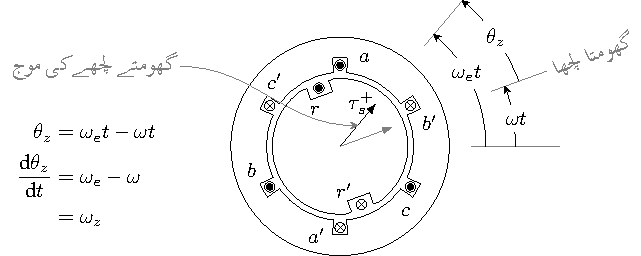
\includegraphics{figInductionStatorAndRotorWaves}
\caption{امالی موٹر اور اس کے گھومتے مقناطیسی دباؤ کی موجیں۔}
\label{شکل_امالی_گھومتی_موجیں}
\end{figure}

گھومتے لچھے بھی بالکل اسی طرح ہوتے ہیں اگرچہ شکل میں صرف ایک ہی گھومتا لچھا دکھایا گیا ہے۔مشین \عددیء{f} زاویائی رفتار سے گھوم رہی ہے۔ تصور کریں کہ لمحہ صفر یعنی \عددیء{t=0} پر گھومتے حصہ کا  \عددیء{a} لچھا صفر زاویہ پر ہے، یعنی یہ نقطہ دار اُفقی لکیر پر ہے مزید یہ کہ اس لمحہ ساکن لچھوں کی گھومتی مقناطیسی دباؤ کی موج بھی اسی اُفقی لکیر پر ہے۔ اب کچھ دیر بعد لمحہ \عددیء{t} پر یہ موج زاویہ  \عددیء{\omega_e t} پر ہو گی۔ اتنی دیر میں گھومتا حصہ گھوم کر زاویہ  \عددیء{\omega t} تک پہنچ جائے گا جہاں \عددیء{\omega=2 \pi f}  مشین کی زاویائی میکانی رفتار ہے۔یہ سب شکل میں دکھایا گیا ہے۔لہٰذا لمحہ \عددیء{t} پر موج اور گھومتے لچھے کے درمیان زاویہ \عددیء{\theta_z} یہ ہو گا
\begin{align}
\theta_z=\omega_e t -\omega t
\end{align}
اگرچہ مقناطیسی موج نے \عددیء{\omega_e t} زاویہ طے کیا لیکن گھومتے لچھے کے حوالے سے اس نے صرف  زاویہ \عددیء{(\omega_e t -\omega t)} طے کیا۔اسی طرح گھومتے لچھے کے حوالے سے اس موج کی  اضافی\حاشیہد{\عددیء{\omega_z} لکھتے ہوئے زیر نوشت میں \عددیء{z}،  لفظ اضافی ک حرف ض کی آواز کو ظاہر کرتا ہے۔} زاویائی رفتار\فرہنگ{اضافی!زاویائی رفتار}\فرہنگ{رفتار!اضافی زاویائی}\حاشیہب{relative angular speed} \عددیء{\omega_z} یہ ہو گی۔
\begin{align}
\omega_z=\frac{\dif \theta_z}{\dif t}=\omega_e -\omega
\end{align}
اس کو مساوات \حوالہ{مساوات_امالی-سرک_تعلق_ب} کی مدد سے یوں لکھ سکتے ہیں۔
\begin{align}
\omega_z=2 \pi (f_e-f)=2 \pi s f_e = s \omega_e
\end{align}
یہ مساوات کہتا ہے کہ گھومتے لچھے کے حوالے سے مقناطیسی موج کی رفتار سرک \عددیء{s} پر منحصر ہے۔اس موج کا حیطہ البتہ تبدیل نہیں ہوا۔ اس طرح گھومتے لچھے کے حوالے سے مقناطیسی موج کی مساوات جو کہ مساوات \حوالہ{مساوات_امالی-سرک_تعلق_ب}  میں دی گئی ہے تبدیل ہو کر یہ بن جائے گی۔
\begin{align}
B_{s,rz}^+(\theta,t)&=B_0 \cos (\theta-\omega_z t)=B_0 \cos (\theta -s \omega_e t)
\end{align}
\عددیء{B_{s,rz}^+} میں \عددیء{+} کا نشان  گھڑی کی اُلٹی سمت گھومتی موج کو ظاہر کرتا ہے جبکہ  زیر نوشت میں \عددیء{s,rz}  \حاشیہد{\عددیء{s} لفظ ساکن کے س کو ظاہر کرتا ہے ، \عددیء{r} لفظ رواں کے ر کو ظاہر کرتا ہے اور \عددیء{z}  لفظ اضافی کے ض کو ظاہر کرتا ہے۔} اس بات کی یاد دھیانی کرتا ہے کہ یہ موج ساکن لچھوں کی وجہ سے وجود میں آیا اور اسے گھومتے یعنی رواں لچھوں کے حوالے سے دیکھا جا رہا ہے۔مزید یہ کہ اس مساوات کی تعدد اضافی تعدد \عددیء{\s \omega_e} کے برابر ہے۔

یوں گھومتے لچھوں میں امالی برقی دباؤ مساوات \حوالہ{مساوات_امالی_تین_دور_سائن_نما_برقی_دباؤ}  کی طرح ہی ہو گی مگر ان کی تعدد \عددیء{\omega_z=s \omega_e t} ہو گی یعنی\حاشیہد{\عددیء{e_{arz}} میں  مرحلہ \عددیء{a} ہے۔گھومتے لچھے کو \عددیء{r}  اور اضافی کو \عددیء{z} ظاہر کرتا ہے۔}
\begin{gather}
\begin{aligned}\label{مساوات_امالی_گھومتا_حصہ_تین_دور_سائن_نما_برقی_دباؤ}
e_{arz}(t)&=s \omega_e N_r \phi_0 \cos (s \omega_e t -90\degree)=s E_r \cos (s \omega_e t -90\degree)\\
e_{brz}(t)&=s \omega_e N_r \phi_0 \cos (s \omega_e t +150\degree)= s E_r \cos (s \omega_e t +150\degree)\\
e_{crz}(t)&=s \omega_e N_r \phi_0 \cos (s \omega_e t +30\degree)= s E_r \cos (s \omega_e t +30\degree)
\end{aligned}
\end{gather}
ان مساوات میں \عددیء{N_r}  گھومتے لچھے کے چکر ہیں اور
\begin{align}
E_r=\omega_e N_r \phi_0
\end{align}

اب تصور کریں کہ گھومتے لچھوں کو کسرِ دور کر دیا کیا گیا ہے۔یہ امالی برقی دباؤ گھومتے لچھوں میں برقی رو \عددیء{i_{arz}}\حاشیہد{یہاں \عددیء{r} گھومتے لچھے کو ظاہر کرتا ہے اور \عددیء{z} اس بات کی یاد دھیانی کرتا ہے کہ اس برقی رو کی تعدد، اضافی تعدد ہے۔}  وغیرہ پیدا کرے گی جس کی تعدد \عددیء{s \omega_e} ہو گی۔بالکل ساکن لچھے کی طرح، گھومتے لچھے کی مزاحمت \عددیء{R_r}\حاشیہد{ٹرانسفارمر کی اصطلاح میں ثانوی لچھے  کو زیر نوشت میں \عددیء{2} سے ظاہر کرتے ہیں۔یہاں اسے \عددیء{r} سے ظاہر کیا جاتا ہے۔} اور اس کی امالہ \عددیء{L_r} ہو گی جس کی متعاملیت \عددیء{j s \omega_e L_r} ہو گی۔اسے ہم یوں لکھ سکتے ہیں۔
\begin{align}
j s \omega_e L_r = j s  X_r
\end{align}
جہاں \عددیء{j X_r} کو \عددیء{j \omega_e L_r} کے برابر لیا گیا ہے، یعنی \عددیء{j X_r} اس لچھے کی ساکن حالت میں متعاملیت ہے جب سرک ایک کے برابر ہو۔گھومتے لچھوں میں برقی رو \عددیء{i_{arz}} شکل \حوالہ{شکل_امالی_گھومتی_لچھوں_کا_مساوی_دور}  کی مدد سے حاصل کی جا سکتی ہے جہاں گھومتے  لچھے میں امالی برقی دباؤ \عددیء{e_{arz}(t)} مساوات \حوالہ{مساوات_امالی_گھومتا_حصہ_تین_دور_سائن_نما_برقی_دباؤ}  میں دیا گیا ہے۔
\begin{figure}
\centering
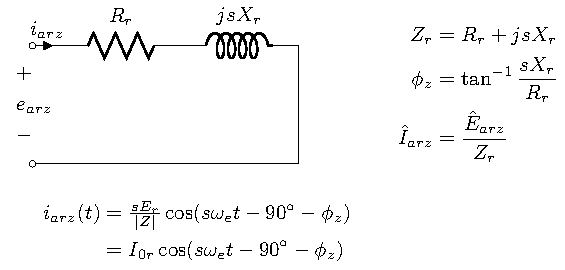
\includegraphics{figInductionRotorEquivalentCircuit}
\caption{گھومتے لچھے کی مساوی دور اور اس میں اضافی تعدد کی رو۔}
\label{شکل_امالی_گھومتی_لچھوں_کا_مساوی_دور}
\end{figure}

یہ شکل بالکل شکل \حوالہ{شکل_حقائق_دوری_سمتیہ_سے_دور_حل}  کی طرح ہے لہٰذا مساوات \حوالہ{مساوات_بنیادی_حقائق_دوری_سمتیہ_سے_مزاحمت_امالہ_دور_حل}  اس میں برقی رو دے گی یعنی
\begin{gather}
\begin{aligned}
i_{arz}(t)&=\frac{s E_r}{\sqrt{R_r^2+s^2 X_r^2}} \cos \left(s \omega_e t -90\degree-\phi_z \right)=I_{0r} \cos (s \omega_e t +\theta_0)\\
i_{brz}(t)&=\frac{s E_r}{\sqrt{R_r^2+s^2 X_r^2}} \cos \left(s \omega_e t +150\degree-\phi_z \right)=I_{0r} \cos (s \omega_e t -120 \degree+\theta_0)\\
i_{crz}(t)&=\frac{s E_r}{\sqrt{R_r^2+s^2 X_r^2}} \cos \left(s \omega_e t +30\degree-\phi_z \right)=I_{0r} \cos (s \omega_e t+120\degree +\theta_0)
\end{aligned}
\end{gather}
یہ تین مرحلہ برقی رو ہیں جو آپس میں \عددیء{120\degree} کا زاویہ رکھتے ہیں۔یہاں \عددیء{\phi_z} رکاوٹ کا زاویہ\حاشیہد{تکنیکی دنیا میں رکاوٹ کے زاویہ کے لئے \عددیء{\phi_z} استعمال ہوتا ہے۔یہاں یہی کیا گیا ہے۔} ہے۔امید کی جاتی ہے کہ اسے آپ مقناطیسی بہاو نہیں سمجھیں گے۔یہاں
\begin{gather}
\begin{aligned}\label{مساوات_امالی_گھومتا_رو}
\theta_0&=-90-\phi_z \\
I_{0r}&=\frac{s E_r}{\sqrt{R_r^2+s^2 X_r^2}}
\end{aligned}
\end{gather}
شکل \حوالہ{شکل_امالی_گھومتی_لچھوں_کا_مساوی_دور}  سے واضح ہے کہ ایک گھومتے لچھے کی مزاحمت میں 
\begin{align}\label{مساوات_امالی_طاقت_ضیاع_گھمتا_حصہ}
p_r =I_{or}^2 R_r
\end{align}
برقی طاقت کا ضیاع ہو گا۔یہ طاقت حرارت میں تبدیل ہو کر اس مزاحمت کو گرم کرے گی۔

\حصہ{گھومتے لچھوں کی گھومتی مقناطیسی دباؤ کی موج}
ہم جانتے ہیں کہ ساکن تین مرحلہ لچھوں میں \عددیء{f_e} تعدد کی برقی رو   گھومتے مقناطیسی دباؤ کی موج کو جنم دیتی ہے جو اس ساکن لچھے کے حوالے سے  \عددیء{f_e} معاصر زاویائی رفتار سے گھومتی ہے۔ اسی طرح گھومتے تین دور لچھوں میں \عددیء{s f_e} تعدد کی برقی رو ایک گھومتی مقناطیسی دباؤ کی موج \عددیء{\tau_{rz}^+} کو جنم دیتی ہے جو اس گھومتے لچھے کے حوالے سے \عددیء{s f_e}  زاویائی رفتار سے گھومتی ہے۔
\begin{align}
\tau_{rz}^+(\theta,t)=k_w \frac{4}{\pi} \frac{N_r I_{0r}}{2} \cos \left(\theta-s \omega_e t -\theta_0 \right)
\end{align}
یہاں  \عددیء{I_{0r}} اور \عددیء{\theta_0} مساوات \حوالہ{مساوات_امالی_گھومتا_رو} میں دیئے گئے ہیں۔اب چونکہ گھومتا لچھا از خود \عددیء{f} زاویائی رفتار سے گھوم رہا ہے لہٰذا اس کی پیدا کردہ مقناطیسی دباؤ کی موج خلاء میں \عددیء{(f+s f_e)} زاویائی رفتار سے گھومتی ہے۔ اس رفتار کو مساوات \حوالہ{مساوات_امالی_سرک_اور_تعدد}  کی مدد سے یوں لکھ سکتے ہیں۔
\begin{align}
f+s f_e= f_e (1-s)+ s f_e=f_e
\end{align}
لہٰذا گھومتے لچھوں کی مقناطیسی دباؤ کی موج کو ساکن لچھوں کے حوالے سے یوں لکھا جا سکتا ہے۔
\begin{align}\label{مساوات_امالی_گھومتے_حصے_کی_موج}
\tau_{r,s}^+(\theta,t)=k_w \frac{4}{\pi} \frac{N_r I_{0r}}{2} \cos \left(\theta-\omega_e t -\theta_0 \right)
\end{align}
\عددیء{\tau_{r,s}^+} میں \عددیء{+} کا نشان گھڑی کی اُلٹی سمت گھومتی موج کو ظاہر کرتا ہے جبکہ زیر نوشت  میں \عددیء{r,s} اس بات کی وضاحت کرتا ہے کہ یہ موج گھومتے یعنی رواں لچھوں کی وجہ سے وجود میں آیا ہے مگر اسے ساکن لچھوں کے حوالے سے دیکھا جا رہا ہے۔

یہاں وقفہ لے کر ذرا غور کرتے ہیں۔مساوات \حوالہ{مساوات_امالی_گھومتے_حصے_کی_موج}  کے مطابق گھومتا لچھا خود کسی بھی رفتار سے گھوم رہا ہو، اس کی پیدا کردہ گھومتی مقناطیسی دباؤ کی موج ساکن لچھے کے پیدا کردہ موج کی رفتار سے ہی گھومے گی۔لہٰذا مشین میں دو گھومتی مقناطیسی دباؤ کی موجیں ہیں جو ایک ہی معاصر رفتار سے گھوم رہی ہیں۔مساوات \حوالہ{مساوات_گھومتے_مشین_مروڑ_کوتوانائی_سے}  میں کہا گیا ہے کہ دو مقناطیسی دباؤ کی موجودگی  پیدا کرتی ہیں جو ان کے مابین زاویہ پر منحصر ہے۔لہٰذا امالی مشین میں موجود دو مقناطیسی موجیں  پیدا کرتی ہیں اور اس  کی مقدار ان دو موجوں کے مابین زاویہ پر منحصر ہوتی ہے۔امالی موٹر اس پر لدے بوجھ کے مطابق ان دو موجوں کے مابین زاویہ رکھتی ہے اور یوں درکار  پیدا کرتی ہے۔

\حصہ{گھومتے لچھوں کے مساوی فرضی ساکن لچھے}
اب دوبارہ اصل موضوع پر آتے ہیں۔اگر گھومتے لچھوں کی جگہ \عددیء{N_r} چکر کے تین مرحلہ فرضی ساکن لچھے ہوں تو مساوات \حوالہ{مساوات_امالی_تین_دور_سائن_نما_برقی_دباؤ}   کی طرح ان میں امالی برقی دباؤ پیدا ہو گی یعنی\حاشیہد{ان مساوات میں زیر نوشت میں \عددیء{f} لفظ فرضی کے ف کو ظاہر کرتا ہے۔}
\begin{gather}
\begin{aligned}\label{مساوات_امالی_تین_دباؤ}
e_{afs}(t)&=\omega_e N_r \phi_0 \cos \left(\omega_e t -90\degree \right)=E_r \cos \left(\omega_e t -90\degree \right)\\
e_{bfs}(t)&=\omega_e N_r \phi_0 \cos \left(\omega_e t +150\degree \right)=E_r \cos \left(\omega_e t +150\degree \right)\\
e_{cfs}(t)&=\omega_e N_r \phi_0 \cos \left(\omega_e t +30\degree \right)=E_r \cos \left(\omega_e t +30\degree \right)
\end{aligned}
\end{gather}
%
\begin{figure}
\centering
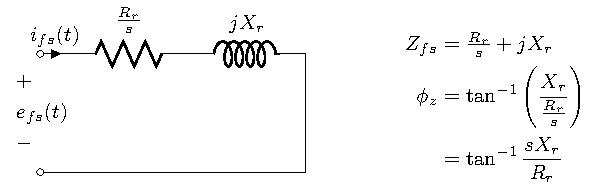
\includegraphics{figInductionRotorEquivalentStaticCircuit}
\caption{گھومتے لچھوں کی جگہ فرضی ساکن لچھے کی دور۔}
\label{شکل_امالی_گھومتی_لچھوں_کا_فرضی_مساوی_ساکن_دور}
\end{figure}

مزید فرض کریں کہ ان فرضی ساکن لچھوں کی مزاحمت \عددیء{\tfrac{R_r}{s}}  اور متعاملیت  \عددیء{j X_r} ہیں  یعنی
\begin{align}
Z_{fs}=\frac{R_r}{s}+j X_r
\end{align}
اگر ان پر مساوات \حوالہ{مساوات_امالی_تین_دباؤ}  میں دیئے گئے برقی دباؤ لاگو کی جائے جیسے شکل \حوالہ{شکل_امالی_گھومتی_لچھوں_کا_فرضی_مساوی_ساکن_دور}  میں دکھایا گیا ہے تو ان میں برقی رو یہ ہو گی۔
\begin{gather}
\begin{aligned}
i_{afs}(t)&=\frac{E_r}{\sqrt{\left(\frac{R_r}{s} \right)^2+X_r^2}} \cos \left(\omega_e t-90\degree -\phi_Z  \right)=I_{or} \cos \left(\omega_e t+\theta_0 \right)\\
i_{bfs}(t)&=\frac{E_r}{\sqrt{\left(\frac{R_r}{s} \right)^2+X_r^2}} \cos \left(\omega_e t+150\degree -\phi_Z  \right)=I_{or}\cos \left(\omega_e t-120\degree +\theta_0 \right)\\
i_{cfs}(t)&=\frac{E_r}{\sqrt{\left(\frac{R_r}{s} \right)^2+X_r^2}} \cos \left(\omega_e t+300\degree -\phi_Z  \right)=I_{or} \cos \left(\omega_e t+120\degree+\theta_0 \right)
\end{aligned}
\end{gather}
یہاں مساوات \حوالہ{مساوات_امالی_گھومتا_رو}  استعمال کی گئی ہے۔اس مساوات میں دھیان رہے کہ رکاوٹ کا زاویہ \عددیء{\phi_Z}  وہی ہے جو گھومتے لچھے کا تھا یعنی
\begin{align}
\phi_{fZ}=\tan^{-1} \frac{X}{\left(\frac{R}{s} \right)}=\tan^{-1} \frac{s X}{R}=\phi_Z
\end{align}
ان برقی رو کی تعدد \عددیء{\omega_e} ہے اور ان کا پیدا کردہ گھومتا مقناطیسی موج یہ ہو گا۔
\begin{align}
\tau_{fs,s}^+(\theta,t)=k_w \frac{4}{\pi}\frac{N_r I_{0r}}{2} \cos (\theta-\omega_e t-\theta_0)
\end{align}
یہ مقناطیسی موج ہو بہو گھومتے لچھے کی موج \عددیء{\tau_{r,s}^+(\theta,t)} ہے ۔

\حصہ{امالی موٹر کا مساوی برقی دور}
ہم ٹرانسفارمر کی ابتدائی جانب لچھے کی برقی دور پہلے بنا چکے ہیں جہاں  لچھے کی مزاحمت \عددیء{R_1} اور اس کی رستا متعاملیت\فرہنگ{رستا متعاملیت}\حاشیہب{leakage reactance}  \عددیء{j X_1} تھی۔ ٹرانسفارمر کے قالب  میں وقت کے ساتھ بدلتی مقناطیسی بہاو اس لچھے میں امالی برقی دباؤ \عددیء{\hat{E}_1} پیدا کرتی۔ یوں 
\begin{align}
\hat{V}_1=\hat{I}_1 \left(R_1+j X_1 \right) +\hat{E}_1
\end{align}
لکھا جا سکتا ہے  جہاں \عددیء{\hat{V}_1} ابتدائی لچھے پر لاگو بیرونی برقی دباؤ ہے۔ہم دیکھیں گے کہ امالی موٹر کے ساکن لچھے کے لئے بھی یہی مساوات حاصل ہو گی۔
\begin{figure}
\centering
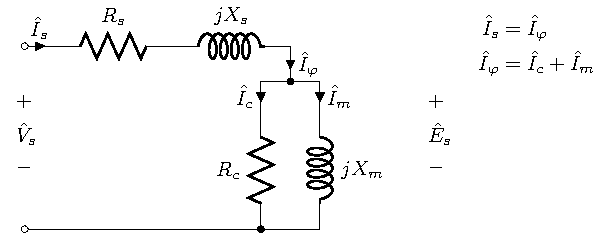
\includegraphics{figInductionStatorEquivalentCircuit}
\caption{امالی موٹر کے ساکن لچھوں کا مساوی برقی دور۔}
\label{شکل_امالی_ساکن_لچھوں_کی_مساوی_دور}
\end{figure}

 تصور کریں کہ مشین کے گھومتے لچھے کھلے دور ہیں اور اس کے ساکن لچھوں پر تین مرحلہ برقی دباؤ لاگو ہے۔ اس صورت میں ساکن لچھوں میں رواں برقی رو ایک گھومتے مقناطیسی دباؤ کی موج \عددیء{\tau_{s}^+(\theta,t)}  پیدا کرے گی جو مساوات \حوالہ{مساوات_امالی_گھومتا_مقناطیسی_دباؤ_الف} میں دی گئی ہے۔

باب کے اس حصہ میں ہم مشین کے ایک مرحلے کو مدِ نظر رکھیں گے، مثلاً مرحلہ \عددیء{a} ۔ یہاں شکل  \حوالہ{شکل_امالی_ساکن_لچھوں_کی_مساوی_دور} سے رجوع کریں۔اگر ساکن لچھے کی مزاحمت \عددیء{R_s} اور متعاملیت \عددیء{j X_s} ہو اور اس پر لاگو بیرونی برقی دباؤ \عددیء{v_s(t)} ہو تو \اصطلاح{کرخوف}\حاشیہب{Kirchoff's voltage law} کے برقی دباؤ کے قانون کے تحت
\begin{align}
v_s(t)=i_s R_s +L_s \frac{\dif i_s}{\dif t}+e_s(t)
\end{align}
\عددیء{e_s(t) } مساوات \حوالہ{مساوات_امالی_تین_دور_سائن_نما_برقی_دباؤ}  میں دی گئی اس موج کی ساکن لچھے میں پیدا امالی برقی دباؤ ہے ۔اسی کو مرحلی سمتیہ کے طور پر یوں لکھ سکتے ہیں۔
\begin{align}\label{مساوات_امالی_دوری_موٹر_مساوات}
\hat{V}_s=\hat{I}_s \left(R_s+j X_s \right)+\hat{E}_s
\end{align}
ٹرانسفارمر کی مثال آگے بڑھاتے ہیں۔اگر موٹر کا گھومتا لچھا کھلے دور\حاشیہب{open circuited} رکھا جائے تو قالب میں ایک ہی گھومتی مقناطیسی دباؤ کی موج \عددیء{\tau_s^+(\theta,t)} ہو گی۔ساکن لچھے میں صرف برقی رو \عددیء{\hat{I}_\varphi} ہو گا جو قالب میں مقناطیسی بہاو \عددیء{\varphi_s} کو جنم دے گی۔ یہ برقی رو \عددیء{\hat{I}_\varphi} غیر سائن نما ہوتی ہے۔ \اصطلاح{فورئیر} تسلسل\حاشیہب{Fourier series} سے اس کے بنیادی جزو اور ہارمونی جزو معلوم کئے جا سکتے ہیں۔ اس کے بنیادی جزو کے دو حصے ہوتے ہیں۔ ایک حصہ  \عددیء{\hat{I}_c}، لاگو بیرونی برقی دباؤ \عددیء{\hat{V}_s} کے ہم قدم ہوتا ہے اور یہ قالب میں طاقت کے ضیاع کو ظاہر کرتا ہے اور دوسرا حصہ \عددیء{\hat{V}_s} سے نوے درجہ پیچھے زاویہ پر رہتا ہے۔\عددیء{\hat{I}_\varphi}میں سے \عددیء{\hat{I}_c} منفی کر کے بقایا کو مقناطیسی جزو کہتے ہیں اسے \عددیء{\hat{I}_m} سے ظاہر کرتے ہیں۔ یوں مقناطیسی جزو بنیادی جزو کے پیچھے حصے اور باقی سارے ہارمونی جزو کے مجموعے پر مشتمل ہوتا ہے اور یہ قالب میں مقناطیسی بہاو \عددیء{\varphi_s} پیدا کرتا ہے۔
\begin{align}
\hat{I}_\varphi=\hat{I}_c+\hat{I}_m
\end{align}
 امالی موٹر کے مساوی دور میں \عددیء{\hat{I}_c} کو مزاحمت \عددیء{R_c} سے اور \عددیء{\hat{I}_m} کو \عددیء{j X_\varphi} سے ظاہر کیا جاتا ہے۔ ان دونوں کا حساب چلتے موٹر میں متوقع برقی تعدد  اور امالی برقی دباؤ \عددیء{\hat{E}_s} پر کیا جاتا ہے یعنی
\begin{gather}
\begin{aligned}
R_c&=\frac{\hat{E}_s}{\hat{I}_c}=\frac{E_s}{I_c}\\
X_\varphi&=\frac{\abs{\hat{E}_s}}{\abs{\hat{I}_m}}=\frac{E_s}{I_m}
\end{aligned}
\end{gather}
مقناطیسی دباؤ کی موج \عددیء{\tau_s^+(\theta,t)} گھومتے لچھے میں بھی امالی برقی دباؤ پیدا کرے گی۔مساوات \حوالہ{مساوات_امالی_دوری_موٹر_مساوات}  میں اگر رکاوٹ میں برقی دباؤ کے گھٹنے کو نظر انداز کیا جائے تو لاگو بیرونی برقی دباؤ اور لچھے کی اندرونی امالی برقی دباؤ ہر حالت میں برابر ہوں گے۔اب تصور کریں کہ گھومتے لچھے کسرِ دور کر دیے جائیں۔ ایسا کرتے ہی ان میں برقی رو گزرنے لگے گا جو مقناطیسی دباؤ کی موج  \عددیء{\tau_{r,s}^+(\theta,t)} جو مساوات \حوالہ{مساوات_امالی_گھومتے_حصے_کی_موج}  میں دی گئی ہے کو جنم دے گی۔ اس موج سے ساکن لچھے میں امالی برقی دباؤ \عددیء{\hat{E}_s} تبدیل ہو جائے گی اور یوں یہ لاگو برقی دباؤ کے برابر نہیں رہے گی۔ یہ ایک نا ممکنہ صورتِ حال ہے۔

ساکن لچھے میں امالی برقی دباؤ،  لاگو برقی دباؤ کے برابر تب رہے گی کہ قالب میں مقناطیسی دباؤ تبدیل نہ ہو۔ مشین کے قالب میں مقناطیسی دباؤ برقرار یوں رہتی ہے کہ ساکن لچھے  مقناطیسی دباؤ \عددیء{\tau_{r,s}^+(\theta,t)}  کی متضاد مقناطیسی دباؤ کی ایک موج پیدا کرتی ہے جو اس کے اثر کو مکمل طور پر ختم کر دیتی ہے۔یہ موج پیدا کرنے کے لئے ساکن لچھوں میں برقی رو \عددیء{\hat{I}_\varphi} سے بڑھ کر \عددیء{(\hat{I}_\varphi+\hat{I}_r')} ہو جاتی ہے جہاں یہ اضافی برقی رو یہ ہیں۔
\begin{gather}
\begin{aligned}\label{مساوات_امالی_تین_رو_الف}
i_{ar}'(t)&=I_{or}' \cos (\omega_e t+\theta_0)\\
i_{br}'(t)&=I_{or}' \cos (\omega_e t-120\degree+\theta_0)\\
i_{cr}'(t)&=I_{or}' \cos (\omega_e t+120\degree+\theta_0)
\end{aligned}
\end{gather}
ان اضافی برقی رو کی متضاد مقناطیسی دباؤ کی موج یہ ہے
\begin{align}
\tau_{(r)}^+(\theta,t)=k_w \frac{4}{\pi}\frac{N_s I_{0r}'}{2} \cos (\theta-\omega_e t -\theta_0)
\end{align}
ساکن لچھوں میں اضافی برقی رو نے ہر لمحہ گھومتے لچھوں کی برقی رو کے اثر کو ختم کرنا ہے لہٰذا یہ دونوں برقی رو ہم قدم\حاشیہب{in-phase} ہی ہوں گے۔چونکہ یہ مساوات اور مساوات \حوالہ{مساوات_امالی_گھومتے_حصے_کی_موج}  برابر ہیں
\begin{align}
N_s I_{0r}'=N_r I_{0r}
\end{align}
 لہٰذا ان سے حاصل ہوتا ہے۔
\begin{align}
I_{0r}'&=\left(\frac{N_r}{N_s}\right) I_{0r}=\left(\frac{N_r}{N_s}\right) \frac{s E_r}{\sqrt{R_r^2+s^2 X_r^2}}
\end{align}
آپ نے دیکھا کہ گھومتے لچھے مقناطیسی دباؤ کی موج پیدا کرتے ہیں جن کے ذریعہ ساکن لچھوں کو معلوم ہوتا ہے کہ موٹر پر بوجھ لدا ہے اور وہ اس کے مطابق لاگو برقی دباؤ سے برقی رو لیتی ہیں۔یہاں تک امالی موٹر کی مساوی برقی دور شکل \حوالہ{شکل_امالی_ساکن_کا_مساوی_دور_بمع_گھومتے_لچھے_کی_رو}  میں دکھائی گئی ہے۔
\begin{figure}
\centering
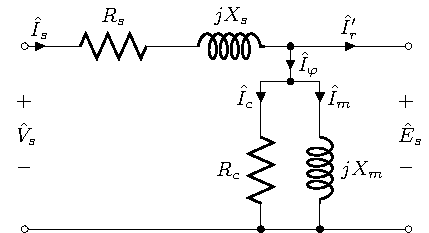
\includegraphics{figInductionStatorEquivalentCircuitWithRotorCurrent}
\caption{مساوی دور اضافی برقی رو کے ساتھ۔}
\label{شکل_امالی_ساکن_کا_مساوی_دور_بمع_گھومتے_لچھے_کی_رو}
\end{figure}

یہاں ذرہ شکل \حوالہ{شکل_امالی_گھومتے_لچھے_کا_دوسرا_مساوی_دور}  سے رجوع کریں۔ اس شکل میں
\begin{figure}
\centering
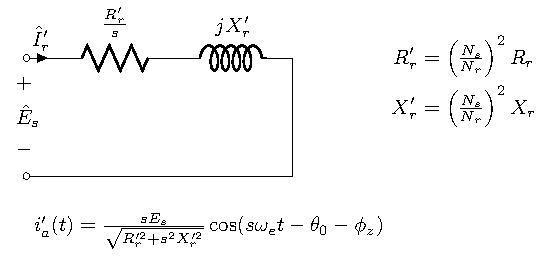
\includegraphics{figInductionRotorEquivalentAnotherCircuit}
\caption{گھومتے لچھے کا ایک اور مساوی دور۔}
\label{شکل_امالی_گھومتے_لچھے_کا_دوسرا_مساوی_دور}
\end{figure}
%
\begin{gather}
\begin{aligned}\label{مساوات_امالی_گھومتے_مزاحمت_امالہ_دوسری_جانب}
R_r'&=\left(\frac{N_s}{N_r} \right)^2 R_r\\
X_r'&=\left(\frac{N_s}{N_r} \right)^2 X_r
\end{aligned}
\end{gather} 
پر ساکن لچھوں کی امالی برقی دباؤ \عددیء{\hat{E}_s} لاگو ہے لہٰذا ان میں برقی رو یہ ہوں گی۔
\begin{gather}
\begin{aligned}\label{مساوات_امالی_تین_رو}
i_a'(t)&=\frac{s E_s}{\sqrt{R_r'^2+s^2 X_r'^2}} \cos (\omega_e t -90\degree -\phi_Z)\\
i_b'(t)&=\frac{s E_s}{\sqrt{R_r'^2+s^2 X_r'^2}} \cos (\omega_e t +150\degree -\phi_Z)\\
i_c'(t)&=\frac{s E_s}{\sqrt{R_r'^2+s^2 X_r'^2}} \cos (\omega_e t +30\degree -\phi_Z)
\end{aligned}
\end{gather}
ان سب مساوات کا حیطہ برابر ہے۔اس حیطے کو یوں لکھا جا سکتا ہے۔
\begin{align}\label{مساوات_امالی_رو_دباؤ_تعلق_الف}
\frac{s E_s}{\sqrt{R_r'^2+s^2 X_r'^2}}=\frac{s \omega_e N_s \phi_0}{\sqrt{\left( \frac{N_s}{N_r}\right)^2 \left(R_r^2+s^2X_r^2 \right)}}=\left(\frac{N_r}{N_s}\right) I_{0r}=I_{0r}'
\end{align}
لہٰذا مساوات \حوالہ{مساوات_امالی_تین_رو}  اس طرح لکھا جاسکتا ہے۔
\begin{gather}
\begin{aligned}
i_a'(t)&=I_{0r}' \cos (\omega_e t -90\degree -\phi_Z)\\
i_b'(t)&=I_{0r}' \cos (\omega_e t +150\degree -\phi_Z)\\
i_c'(t)&=I_{0r}' \cos (\omega_e t +30\degree -\phi_Z)
\end{aligned}
\end{gather}
یہ مساوات بالکل مساوات \حوالہ{مساوات_امالی_تین_رو_الف}  کی طرح ہے۔ لہٰذا اگر شکل \حوالہ{شکل_امالی_ساکن_کا_مساوی_دور_بمع_گھومتے_لچھے_کی_رو}  میں ساکن لچھوں کی امالی برقی دباؤ \عددیء{\hat{E}_s} کے متوازی شکل \حوالہ{شکل_امالی_گھومتے_لچھے_کا_دوسرا_مساوی_دور}  جوڑا جائے تو ایسا کرنے سے ساکن لچھوں میں اُتنا ہی اضافی برقی رو رواں ہو گا جو اصل موٹر میں گھومتے لچھوں کی وجہ سے ہوتا ہے۔ شکل \حوالہ{شکل_امالی_مشین_کا_مکمل_مساوی_دور}  میں ایسا ہی کیا گیا ہے لہٰذا شکل میں دیا برقی دور، امالی موٹر کی صحیح عکاسی کرتی ہے۔ یہی امالی موٹر کی مساوی برقی دور ہے۔
\begin{figure}
\centering
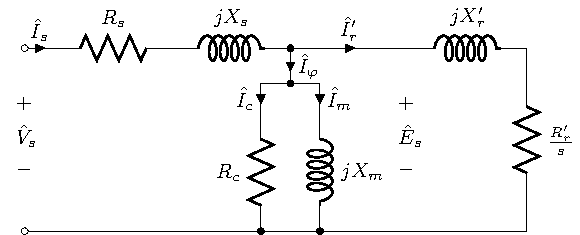
\includegraphics{figInductionMachineEquivalentCircuit}
\caption{امالی موٹر کی مساوی برقی دور۔}
\label{شکل_امالی_مشین_کا_مکمل_مساوی_دور}
\end{figure}


\حصہ{مساوی برقی دور پر غور}
مساوات \حوالہ{مساوات_امالی_طاقت_ضیاع_گھمتا_حصہ}  ایک گھومتے لچھے میں برقی طاقت کے ضیاع کو ظاہر کرتا ہے۔مساوات \حوالہ{مساوات_امالی_گھومتے_مزاحمت_امالہ_دوسری_جانب}  اور \حوالہ{مساوات_امالی_رو_دباؤ_تعلق_الف}   کی مدد سے اسے یوں لکھا جا سکتا ہے۔
\begin{align}
p_{\textup{ضیاع}}&=I_{0r}^2 R_r=\left(\frac{N_s^2}{N_r^2} I_{0r}'^2 \right) \left (\frac{N_r^2}{N_s^2} R_r' \right)=I_{0r}'^2 R_r'
\end{align}
شکل \حوالہ{شکل_امالی_مشین_کا_مکمل_مساوی_دور}  سے ظاہر ہے کہ ایک گھومتے لچھے کو کُل
\begin{align}\label{مساوات_امالی_میکانی_طاقت_بالمقابل_سرک_الف}
p_r = I_{0r}'^2 \frac{R_r'}{s}
\end{align}
برقی طاقت دی جاتی ہے جس میں سے \عددیء{p_{\textup{ضیاع}}} گھومتے لچھے کی مزاحمت میں ضائع ہو جاتی ہے اور بقایا بطور میکانی طاقت  مشین کے دھرے پر پائی جاتی ہے یعنی
\begin{align}
p=I_{0r}'^2 \frac{R_r'}{s}-I_{0r}'^2 R_r'=I_{0r}'^2 \frac{R_r'}{s} (1-s)=p_r (1-s)
\end{align}
یوں  تین مرحلہ مشین جس میں تین لچھے ہوتے ہیں  اس کے تین گنا میکانی طاقت فراہم کر سکتی ہے یعنی
\begin{align}\label{مساوات_امالی_تین_دور_میکانی_طاقت_بالمقابل_سرک_الف}
p_{\textup{میکانی}} =3 I_{0r}'^2 \frac{R_r'}{s} (1-s)=3 p_r (1-s)
\end{align}
 اس مساوات سے واضح ہے کہ اگر سرک ایک کے برابر ہو تو موٹر کوئی میکانی طاقت فراہم نہیں کرے گی اور گھومتے حصے کو جتنی برقی توانائی مل رہی ہو وہ ساری کی ساری اس میں ضائع ہو کر اسے گرم کرے گی۔ یوں موٹر کے گرم ہو کر جل جانے کا امکان ہوتا ہے۔ آپ اس مساوات سے دیکھ سکتے ہیں کہ امالی موٹر کی سرک صفر کے قریب رہنی چاہئے ورنہ یہ ناقابلِ قبول حد تک برقی توانائی ضائع کرے گا۔ ہم امالی موٹر کی مساوی برقی دور کو شکل \حوالہ{شکل_امالی_مشین_کا_دوسرا_مکمل_مساوی_دور}  کی طرح بھی بنا سکتے ہیں۔ اس شکل میں شکل \حوالہ{شکل_امالی_مشین_کا_مکمل_مساوی_دور}  میں دیئے مزاحمت  \عددیء{\tfrac{R_r'}{s}} کو دو حصوں میں لکھا گیا ہے یعنی
\begin{align*}
\frac{R_r'}{s}=R_r'+ R_r' \left( \frac{1-s} {s}\right)
\end{align*}
یوں شکل \حوالہ{شکل_امالی_مشین_کا_مکمل_مساوی_دور}  میں مزاحمت  \عددیء{R_r'} میں برقی طاقت کی ضیاع \عددیء{I_{0r}'^2 R_r'} گھومتے لچھے کی ضیاع ہے جبکہ مزاحمت \عددیء{R_r' \left(\tfrac{1-s}{s} \right)} میں برقی طاقت کی ضیاع \عددیء{I_{0r}'^2 R_r' \left(\tfrac{1-s}{s} \right)} دراصل میکانی طاقت  ہے۔یاد رہے کہ تین مرحلہ  مشین کے لئے یہاں سے حاصل نتائج کو تین سے ضرب دینا ہو گا۔
\begin{figure}
\centering
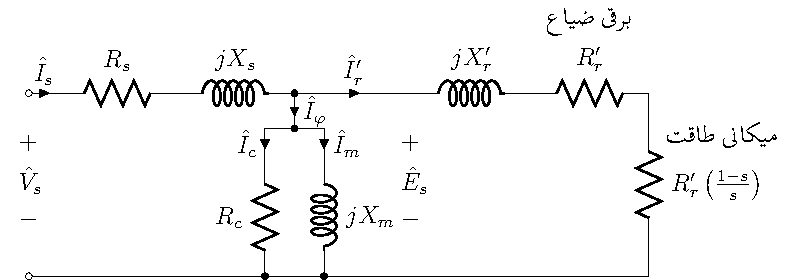
\includegraphics{figInductionMachineAnotherEquivalentCircuit}
\caption{امالی موٹر کی ایک اور مساوی برقی دور۔}
\label{شکل_امالی_مشین_کا_دوسرا_مکمل_مساوی_دور}
\end{figure}

میکانی طاقت، قوت گردشہ ضربِ میکانی زاویائی رفتار ہوتی ہے۔ امالی موٹر کی میکانی زاویائی رفتار مساوات \حوالہ{مساوات_امالی_سرک_اور_تعدد}  میں دی گئی ہے جبکہ مساوات \حوالہ{مساوات_گھومتے_مشین_برقی_میکانی_رفتار_تعلق}  میں میکانی معاصر رفتار \عددیء{\omega_{sm}} دی گئی ہے۔یوں
\begin{align}\label{مساوات_امالی_تین_دور_میکانی_طاقت_اور_رفتار}
p= T_m \omega =T_m \times 2 \pi f=T_m \times 2 \pi (1-s) f_s=T_m (1-s) \omega_{sm} 
\end{align}
لہٰذا
\begin{align}\label{مساوات_امالی_مروڑ_الف}
T_m=\frac{p}{(1-s) \omega_{sm}}=\frac{3 I_{0r}'^2}{\omega_{sm}} \frac{R_r'}{s}
\end{align}
اصل موٹر میں رگڑ، قالبی ضیاع، لچھوں میں ضیاع اور دیگر وجوہات کی بنا پر دھرے پر طاقت یا قوت گردشہ اس سے قدرِ کم ہو گی۔

ٹرانسفارمر کے سادہ ترین مساوی دور بناتے وقت \عددیء{R_c} اور \عددیء{X_m} کو نظرانداز کیا گیا تھا۔ امالی موٹر میں ایسا کرنا ممکن نہیں ہوتا چونکہ موٹروں میں خلائی درز ہوتی ہے جس میں مقناطیسی بہاو پیدا کرنے کے لئے بہت زیادہ مقناطیسی دباؤ درکار ہوتی ہے۔حقیقت میں بے بوجھ امالی موٹر کو اپنے پورے برقی رو کے تیس سے پچاس فی صد برقی رو قالب کو ہیجان کرنے کے لئے درکار ہوتی ہے۔ مزید یہ کہ خلائی درز کی وجہ سے اس کی رِستا امالہ بھی زیادہ ہوتی ہے اور اسے نظر انداز کرنا ممکن نہیں ہوتا۔ البتہ مساوی دور میں \عددیء{R_c} کو نظرانداز کیا جا سکتا ہے جیسے شکل \حوالہ{شکل_امالی_ساکن_حصے_کا_تھونن_دور} میں دکھایا گیا ہے۔ اس شکل میں نقطہ دار لکیر کی بائیں جانب کا مساوی تھوِنن دور بنایا جا سکتا ہے۔ایسا کرنے سے امالی موٹر پر غور کرنا نہایت آسان ہو جاتا ہے۔ اب ہم ایسا ہی کرتے ہیں۔
\begin{figure}
\centering
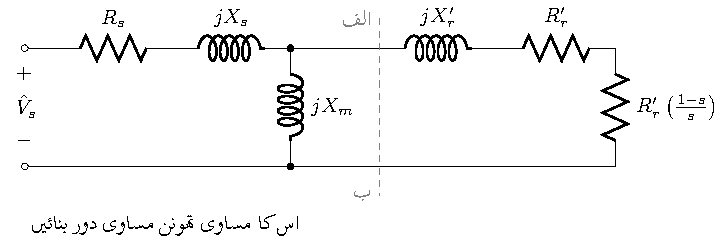
\includegraphics{figInductionMachineTheveninNeededOfStatorSide}
\caption{امالی موٹر کا سادہ دور۔ قالبی ضیاع کو نظرانداز کیا گیا ہے۔}
\label{شکل_امالی_ساکن_حصے_کا_تھونن_دور}
\end{figure}
%
\ابتدا{مثال}\شناخت{مثال_امالی_ستارہ_چھ_قطب_پندرہ_کلو_واٹ}
ستارہ جڑی چھ قطب پچاس ہرٹز اور  \عددیء{415} وولٹ پر چلنے والی  \عددیء{15} کلو واٹ امالی موٹر کے مساوی دور کے اجزاء یہ ہیں
\begin{align*}
R_s= \SI{0.5}{\ohm}, \quad R_r'=\SI{0.31}{\ohm}, \quad X_s=\SI{0.9}{\ohm}, \quad X_r'=\SI{0.34}{\ohm}, \quad X_m=\SI{0.22}{\ohm} 
\end{align*}
موٹر میں رگڑ سے طاقت کا ضیاع  \عددیء{600} واٹ ہے۔قالبی ضیاع کو اسی کا حصہ تصور کیا گیا ہے۔ اس کو اٹل تصور کیا جائے۔یہ موٹر درکار وولٹ اور تعداد ارتعاش پر دو فی صد سرک پر چل رہی ہے۔اس حالت میں موٹر کی رفتار، اس کے دھرے پر پیدا قوت گردشہ اور طاقت، اس کے ساکن لچھے کی برقی رو اور اس کی فی صد کارگزاری حاصل کریں۔

حل:
موٹر کی معاصر رفتار \عددیء{f_m=\tfrac{2}{6} \times 50=16.66} چکر فی سیکنڈ یا \عددیء{16.66\times 60=1000} چکر فی منٹ۔دو فی صد سرک پر موٹر کی رفتار \عددیء{f=16.66 \times (1-0.02)=16.33} چکر فی سیکنڈ یا  \عددیء{16.33 \times 60=979.8} چکر فی منٹ ہے۔

شکل \حوالہ{شکل_امالی_ساکن_حصے_کا_تھونن_دور}  میں دائیں جانب
\begin{align*}
j X_r'+R_r'+R_r' \frac{1-s}{s}=j X_r'+\frac{R_r'}{s}=j 0.34+\frac{0.31}{0.02}=j 0.34+15.5
\end{align*}
اور \عددیء{j X_m} متوازی جڑے ہیں۔ان کی مساوی رکاوٹ یہ ہے
\begin{align*}
\frac{1}{Z}&=\frac{1}{15.5+j 0.34}+\frac{1}{j 22}\\
Z&=10.147+j 7.375=R+jX
\end{align*}
موٹر پر لاگو  یک مرحلہ برقی دباؤ  \عددیء{\tfrac{415}{\sqrt{3}}=239.6} وولٹ ہے۔ یوں ساکن لچھے کی برقی رو
\begin{align*}
\hat{I}_s&=\frac{\hat{V}_s}{R_s+j X_s+Z}\\
&=\frac{239.6}{0.5+j0.99+10.147+j 7.375}\\
&=17.6956 \phase{-38.155 \degree}
\end{align*}
ہے۔اس موٹر کے گھومتے حصہ کو وہی طاقت منتقل ہو رہی ہے جو رکاوٹ \عددیء{Z}  کو منتقل ہو رہی ہے۔یعنی مساوات \حوالہ{مساوات_امالی_میکانی_طاقت_بالمقابل_سرک_الف} کو ہم یوں بھی لکھ سکتے ہیں۔
\begin{align*}
p=I_{or}'^2 \frac{R_r'}{s}=I_s^2 R=17.6956^2 \times 10.147=\SI{3177.37}{\watt}
\end{align*}
تین مراحل کے لئے  یہ مقدار  \عددیء{3 \times 3177.37=9532} واٹ ہو گی۔مساوات \حوالہ{مساوات_امالی_تین_دور_میکانی_طاقت_بالمقابل_سرک_الف}  موٹر کی اندرونی میکانی طاقت دیتی ہے یعنی
\begin{align*}
p_{\textup{میکانی}}=
9532 \times (1-0.02)=\SI{9341}{\watt}
\end{align*}
اس سے طاقت کا ضیاع منفی کر کے \عددیء{9341-600=8741} واٹ رہ جاتا ہے۔یہ موٹر کے دھرے پر میکانی طاقت ہو گی جس سے دھرے پر قوت گردشہ
\begin{align*}
T=\frac{8741}{2 \times \pi \times 16.33}=\SI{85.1}{\newton \meter}
\end{align*}
ہو گی۔

موٹر کو کُل مہیا برقی طاقت \عددیء{\sqrt{3} \times 415 \times 17.6956 \times \cos (-38.155)=10001.97} واٹ ہے۔ یوں اس موٹر کی کارگزاری  \عددیء{\tfrac{8741}{10001.97} \times 100=\SI{87.39}{\percent}} ہے۔
\انتہا{مثال}
%
\حصہ{امالی موٹر کا مساوی تھونن دور  یا ریاضی نمونہ}
مسئلہ \اصطلاح{تھوِنن}\فرہنگ{مسئلہ!تھونن}\حاشیہب{Thevenin theorem}\فرہنگ{Thevenin theorem} کے مطابق کسی بھی سادہ خطی برقی دور\فرہنگ{خطی!برقی دور}\حاشیہب{linear circuit}\فرہنگ{linear circuit} کو اس کے دو برقی سروں کے مابین ایک رکاوٹ اور ایک برقی دباؤ کی مساوی دور سے ظاہر کیا جا سکتا ہے۔اس مساوی دور کو مساوی تھوِنن دور کہتے ہیں جبکہ اس مساوی تھوِنن دور کی رکاوٹ کو تھوِنن رکاوٹ اور برقی دباؤ کو تھوِنن برقی دباؤ کہتے ہیں۔

برقی دور کے دو برقی سروں کے مابین تھوِنن رکاوٹ حاصل کرنے کے لئے  اس برقی دور کے اندرونی برقی دباؤ کسرِ دور کر کے ان دو برقی سروں کے مابین رکاوٹ معلوم کی جاتی ہے۔یہی رکاوٹ، تھوِنن رکاوٹ ہے۔انہیں برقی سروں پر تھوِنن برقی دباؤ حاصل کرنے کے لئے دیئے گئے برقی دور کے اندرونی برقی دباؤ برقرار رکھ کر ان دو سروں پر برقی دباؤ معلوم کی جاتی ہے۔ یہی برقی دباؤ در حقیقت تھوِنن برقی دباؤ ہے۔بعض اوقات ہم ایک برقی دور کے ایک خاص حصے کا مساوی تھوِنن دور بنانا چاہتے ہیں۔ایسا کرتے وقت بقایا برقی دور کو اس حصے سے مکمل طور پر منقطع کیا جاتا ہے۔
\begin{figure}
\centering
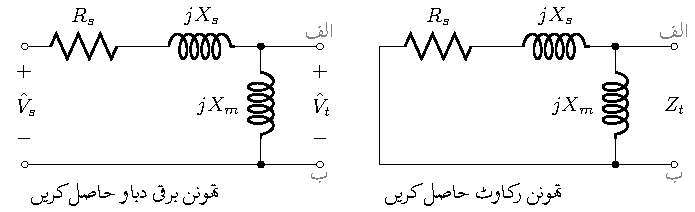
\includegraphics{figInductionMachineTheveninImpedanceAndVoltage}
\caption{تھوِنن رکاوٹ اور تھوِنن برقی دباؤ حاصل کرنے کے دور۔}
\label{شکل_امالی_تھونن_رکاوٹ_اور_دباؤ}
\end{figure}
یوں شکل \حوالہ{شکل_امالی_تھونن_رکاوٹ_اور_دباؤ}  سے واضح ہے کہ دو سروں الف اور با کے مابین مساوی تھوِنن  رکاوٹ اور تھوِنن برقی دباؤ یہ ہیں۔
\begin{gather}
\begin{aligned}\label{مساوات_امالی_تھونن_متغرات}
Z_t&=\frac{\left(R_s+j X_s \right) j X_m}{R_s +j X_s + j X_m}=R_t+j X_t\\
\hat{V}_t&=\frac{j X_m \hat{V}_s}{R_s +j X_s + j X_m}=V_t \phase{\theta_t}
\end{aligned}
\end{gather}
%
\begin{figure}
\centering
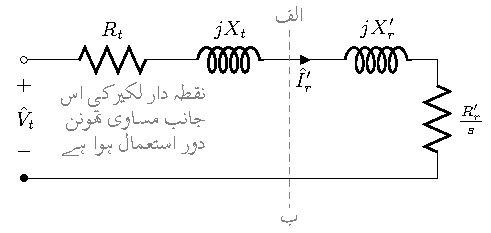
\includegraphics{figInductionMachineUsingThevenin}
\caption{تھوِنن دور استعمال کرنے کے بعد امالی موٹر کا مساوی دور۔}
\label{شکل_امالی_تھونن_استعمال_کرتے_ہوئے}
\end{figure}
کسی بھی مخلوط عدد\حاشیہب{complex number} کی طرح  \عددیء{Z_t} کو ایک حقیقی عدد \عددیء{R_t} اور ایک فرضی عدد \عددیء{j X_t} کا مجموعہ لکھا جا سکتا ہے۔ یہی اس مساوات میں کیا گیا ہے۔

ہم یوں امالی موٹر کی مساوی برقی دور کو شکل \حوالہ{شکل_امالی_تھونن_استعمال_کرتے_ہوئے}  کی طرح بنا سکتے ہیں جہاں سے مرحلی سمتیہ کی استعمال سے مندرجہ ذیل برقی رو \عددیء{\hat{I}_r'} حاصل ہوتی ہے۔
\begin{gather}
\begin{aligned}\label{مساوات_امالی_گھمتا_رو}
\hat{I}_r'&=\frac{\hat{V}_t}{R_t +  j X_t +\frac{R_r'}{s}+ j X_r'}\\
\abs{\hat{I}_r'}&=I_r'=\frac{V_t}{\sqrt{\left(R_t+\frac{R_r'}{s} \right)^2+\left(X_t+X_r' \right)^2}}
\end{aligned}
\end{gather}
چونکہ \عددیء{I_r'} کی قیمت پر \عددیء{\hat{V}_t} کے زاویے کا کوئی اثر نہیں لہٰذا مساوی تھونن دور میں \عددیء{\hat{V}_t} کی جگہ  \عددیء{V \phase{0}} استعمال کیا جا سکتا ہے۔بقایا کتاب میں ایسا ہی کیا جائے گا۔ 

مساوات \حوالہ{مساوات_امالی_مروڑ_الف}  سے یوں تین مرحلہ مشین کی قوت گردشہ یہ ہو گی
\begin{gather}
\begin{aligned}\label{مساوات_امالی_تین_دور_مروڑ_الف}
T&=\frac{1}{\omega_{sm}} \frac{3 V_t^2 \left(\frac{R_r'}{s} \right)}{\left(R_t+\frac{R_r'}{s} \right)^2+\left(X_t+X_r' \right)^2}\\
&=\frac{1}{\omega_{sm}} \frac{3 V_t^2 \left(\frac{R_r'}{s} \right)}{\frac{R_r'^2}{s^2}+2 R_t \frac{R_r'}{s}+R_t^2+\left(X_t+X_r' \right)^2}
\end{aligned}
\end{gather}

اس مساوات کو شکل \حوالہ{شکل_امالی_مروڑ_بالمقابل_رفتار}  میں دکھایا گیا ہے۔ اس شکل میں موٹر کی رفتار کو معاصر رفتار کی نسبت سے دکھایا گیا ہے۔موٹر ازخود گھومتے مقناطیسی موج کی سمت میں گھومتی ہے اور اس کی رفتار معاصر رفتار سے قدرِ کم رہتی ہے۔زیادہ سرک پر موٹر کی کارگزاری نہایت خراب ہو جاتی ہے۔ اسی لئے  لگاتار استعمال کے وقت اسے تقریباً پانچ فی صد سے کم سرک پر چلایا جاتا ہے بلکہ ان کی تخلیق یوں کی جاتی ہے کہ امالی موٹر اپنی پوری طاقت تقریباً پانچ فی صد سے کم سرک پر حاصل کرتی ہے۔ 

اگر موٹر کو زبردستی ساکن لچھوں کی گھومتے مقناطیسی موج کی سمت میں معاصر رفتار سے زیادہ رفتار پر گھمایا جائے تو یہ ایک جنریٹر کے طور پر کام کرنے شروع ہو جائے گی۔ایسا کرنے کے لئے بیرونی میکانی طاقت درکار ہو گی ۔اگرچہ امالی مشین عام طور پر جنریٹر کے طور پر استعمال نہیں ہوتے البتہ ہوا سے برقی طاقت پیدا کرنے میں یہ جنریٹر کے طور پر کار آمد ثابت ہوتے ہیں۔
\begin{figure}
\centering
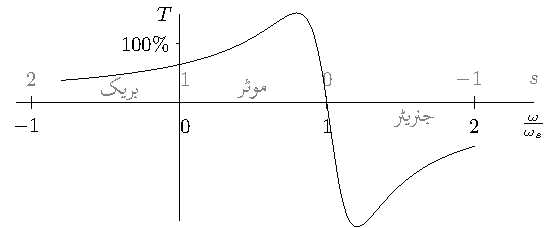
\includegraphics{figInductionTorqueSlip}
\caption{امالی موٹر کی قوت گردشہ بالمقابل سرک کا خط۔}
\label{شکل_امالی_مروڑ_بالمقابل_رفتار}
\end{figure}

شکل \حوالہ{شکل_امالی_مروڑ_بالمقابل_رفتار} میں منفی رفتار بھی دکھائی گئی ہے جہاں سرک ایک سے زیادہ ہے۔ ایسا تب ہوتا ہے جب موٹر کو ساکن لچھوں کی گھومتی مقناطیسی دباؤ کی موج کی اُلٹ سمت میں گھمایا جائے۔موٹر کو جلد ساکن حالت میں لانے کے لئے یوں کیا جاتا ہے۔تین مرحلہ موٹر پر لاگو برقی دباؤ کی کسی دو مرحلوں کو آپس میں اُلٹا دیا جاتا ہے۔ اس طرح موٹر کی ساکن لچھوں کی گھومتی مقناطیسی موج یکدم اُلٹ سمت میں گھومنے شروع ہو جاتی ہے جبکہ موٹر ابھی پہلی سمت میں ہی گھوم رہی ہوتی ہے۔اس طرح موٹر جلد آہستہ ہوتی ہے اور جیسے ہی موٹر رکھ کر دوسری جانب گھومنا چاہتی ہے اس پر لاگو برقی دباؤ منقطع کر دی جاتی ہے۔امالی موٹر یوں ریل  گاڑی میں عموماً بطور بریک\حاشیہب{brake} استعمال کی جاتی ہے۔

یوں امالی مشین \عددیء{s<0} کی صورت میں بطور جنریٹر، \عددیء{0<s<1} کی صورت میں بطور موٹر اور \عددیء{1<s} کی صورت میں بطور بریک کام کرتا ہے۔

امالی موٹر کی زیادہ سے زیادہ قوت گردشہ مساوات \حوالہ{مساوات_امالی_تین_دور_مروڑ_الف}  سے یوں حاصل کی جا سکتی ہے۔قوت گردشہ اُسی لمحہ زیادہ سے زیادہ ہو گی جب گھومتے حصے کو زیادہ سے زیادہ طاقت میسر ہو۔زیادہ سے زیادہ طاقت منتقل کرنے کے مسئلہ\فرہنگ{مسئلہ!زیادہ سے زیادہ طاقت کی منتقلی}\حاشیہب{maximum power theorem}\فرہنگ{theorem!maximum power transfer} کے مطابق مزاحمت \عددیء{\tfrac{R_r'}{s}} میں طاقت کا ضیاع اس وقت زیادہ سے زیادہ ہو گا جب
\begin{align}\label{مساوات_امالی_زیادہ_طاقت_منتقلی_شرط}
\frac{R_r'}{s}=\abs{R_t+j X_t+j X_r'}=\sqrt{R_t^2+\left(X_t+X_r'\right)^2}
\end{align}
ہو۔اس مساوات سے زیادہ سے زیادہ طاقت پر سرک \عددیء{s_z} کو یوں لکھ سکتے ہیں۔
\begin{align}\label{مساوات_امالی_زیادہ_طاقت_پر_سرک}
s_z=\frac{R_r'}{\sqrt{R_t^2+\left(X_t+X_r'\right)^2}}
\end{align}
مساوات \حوالہ{مساوات_امالی_تین_دور_مروڑ_الف}  میں کسر کے نچلے حصے میں \عددیء{R_t^2+(X_t+X_r')^2} کی جگہ  مساوات \حوالہ{مساوات_امالی_زیادہ_طاقت_منتقلی_شرط}  کا مربع استعمال کرتے ہوئے زیادہ سے زیادہ قوت گردشہ  یوں حاصل کی جا سکتی ہے
\begin{gather}
\begin{aligned}
T_z&=\frac{1}{\omega_{sm}} \frac{3 V_t^2 \left(\frac{R_r'}{s} \right)}{\frac{R_r'^2}{s^2}+2 R_t \frac{R_r'}{s}+\frac{R_r'^2}{s^2}}\\
&=\frac{1}{\omega_{sm}} \frac{3 V_t^2 }{2 \left(R_t+\frac{R_r'}{s} \right)}\\
&=\frac{1}{\omega_{sm}} \frac{3 V_t^2}{2 \left(R_t+\sqrt{R_t^2+\left(X_t+X_r' \right)^2} \right)}
\end{aligned}
\end{gather}
جہاں آخری قدم پر مساوات کا استعمال دوبارہ کیا گیا۔

اس مساوات کے مطابق امالی موٹر کی زیادہ سے زیادہ قوت گردشہ اس کے گھومتے لچھوں کی  مزاحمت پر منحصر نہیں۔ یہ ایک اہم معلومات ہے جسے استعمال کر کے امالی موٹر کی زیادہ سے زیادہ قوت گردشہ درکار رفتار پر  حاصل کی جا سکتی ہے۔آئیں دیکھیں کہ یہ کیسا کیا جاتا ہے۔
\begin{figure}
\centering
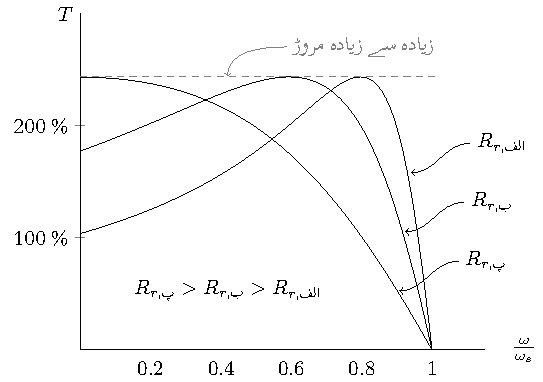
\includegraphics{figInductionTorqueSlipRotorResistanceIncreased}
\caption{بیرونی مزاحمت لگانے کے قوت گردشہ بالمقابل سرک کے خطوط پر اثرات۔}
\label{شکل_امالی_بیرونی_مزاحمت_اور_مروٹ}
\end{figure}

	امالی موٹر کے گھومتے لچھوں کے برقی سروں کو \اصطلاح{سرک چھلوں}\فرہنگ{سرک چھلے}\حاشیہب{slip rings}\فرہنگ{slip rings} کے ذریعہ باہر نکالا جاتا ہے\حاشیہد{شکل  کے نمونے پر۔} جہاں ان کے ساتھ سلسلہ وار بیرونی مزاحمت جوڑی جاتی ہے۔اس طرح گھومتے لچھوں کی کل مزاحمت بڑھ کر \عددیء{R_r + R_{\textup{بیرونی}}} ہو جاتی ہے۔ ایسا کرنے سے مساوات \حوالہ{مساوات_امالی_زیادہ_طاقت_منتقلی_شرط}  کے مطابق زیادہ سے زیادہ قوت گردشہ نسبتاً زیادہ سرک یعنی کم زاویائی رفتار پر حاصل کی جا سکتی ہے۔ شکل \حوالہ{شکل_امالی_بیرونی_مزاحمت_اور_مروٹ} میں مزاحمت \عددیء{R_{r,\textup{پ}}} کے ساتھ ساکن موٹر کو چالو کرتے وقت زیادہ سے زیادہ قوت گردشہ حاصل ہو سکتی ہے۔اس طرح بوجھ بردار موٹر ساکن حالت سے ہی زیادہ بوجھ اٹھانے کے قابل ہوتا ہے۔ چونکہ زیادہ سرک پر موٹر کی کارگزاری خراب ہوتی ہے لہٰذا اس طرح موٹر کو زیادہ دیر نہیں چلایا جاتا اور جیسے ہی اس کی رفتار بڑھ جاتی ہے، اس سے جُڑے بیرونی مزاحمتیں منقطع کر کے گھومتے لچھوں کے برقی سرے کسرِ دور کر دیئے جاتے ہیں۔

\ابتدا{مثال}
صفحہ \حوالہصفحہ{مثال_امالی_ستارہ_چھ_قطب_پندرہ_کلو_واٹ} پر مثال \حوالہ{مثال_امالی_ستارہ_چھ_قطب_پندرہ_کلو_واٹ}  میں دی گئی امالی موٹر اس مثال میں استعمال کریں۔رگڑ سے طاقت کی ضیاع کو نظر انداز کریں۔
\begin{itemize}
\item
اگر موٹر درکار وولٹ اور تعداد ارتعاش پر تین فی صد سرک پر چل رہی ہو تو  ساکن لچھے میں گھومتے لچھے کے حصہ کی برقی رو \عددیء{I_r'} اور مشین کی اندرونی میکانی طاقت اور قوت گردشہ حاصل کریں۔
\item
موٹر کی زیادہ سے زیادہ اندرونی پیدا قوت گردشہ اور اس قوت گردشہ پر موٹر کی رفتار حاصل کریں۔
\item
موٹر کی چالو ہونے کے لمحہ پر قوت گردشہ اور اسی لمحہ اس کی \عددیء{I_r'}  حاصل کریں۔ 
\end{itemize}

حل:
\begin{itemize}
\item
 یک مرحلہ  برقی دباؤ \عددیء{\tfrac{415}{\sqrt{3}}=239.6}  استعمال کرتے ہوئے مساوات \حوالہ{مساوات_امالی_تھونن_متغرات}  کی مدد سے
\begin{align*}
Z_t&=\frac{\left(0.5+j 0.99 \right) j 22}{0.5+j 0.99+j 22}=0.4576+j 0.9573\\
\hat{V}_t&=\frac{j 22 \times 239.6 \phase{0\degree}}{0.5+j 0.99+j 22}=229.2\phase{1.246\degree}
\end{align*}
مساوات \حوالہ{مساوات_امالی_گھمتا_رو}  میں  تین فی صد سرک پر \عددیء{\tfrac{R_r'}{s}=10.3333} کے استعمال سے
\begin{align*}
\hat{I}_r'&=\frac{229.2 \phase{1.246\degree}}{0.4576+j 0.9573+10.3333+j 0.34}=21.1\phase{-5.6\degree}\\
I_r'&=\abs{\hat{I}_r'}=\SI{21.1}{\ampere}
\end{align*}
یہاں رک کر تسلی کر لیں کہ مندرجہ بالا مساوات میں \عددیء{229.2\phase{1.246\degree}} کی جگہ \عددیء{229.2\phase{0\degree}} استعمال کرنے سے \عددیء{I_r'} کی یہی قیمت حاصل ہوتی۔

مساوات \حوالہ{مساوات_امالی_تین_دور_میکانی_طاقت_بالمقابل_سرک_الف}  اور \حوالہ{مساوات_امالی_تین_دور_میکانی_طاقت_اور_رفتار}  کی مدد سے
\begin{align*}
p_m&=\frac{3\times 21.1^2\times 0.31}{0.03} \times (1-0.03)=\SI{13387.46}{\watt}\\
T&=\frac{13387.46}{(1-0.03) \times 2\times \pi \times 16.66}=\SI{131.83}{\newton \meter}
\end{align*}
%
\item
مساوات \حوالہ{مساوات_امالی_زیادہ_طاقت_پر_سرک}  سے زیادہ سے زیادہ طاقت پر سرک
\begin{align*}
s_z=\frac{0.31}{\sqrt{0.4576^2+(0.9573+0.34)^2}}=0.1638
\end{align*}
اور اس پر موٹر کی رفتار \عددیء{1000\times(1-0.1638)=836.2} چکر فی منٹ ہو گی۔
\item
چالو کرتے لمحہ پر سرک ایک ہو گی لہٰذا \عددیء{\tfrac{R_r'}{s}=0.31} ہو گا اور یوں
\begin{align*}
\hat{I}_r'&=\frac{229.2 \phase{1.246\degree}}{0.4576+j 0.9573+0.31+j 0.34}=152.07\phase{-58.14\degree}\\
I_r'&=\SI{152}{\ampere}
\end{align*}
اس لمحہ قوت گردشہ
\begin{align*}
T=\frac{3 \times 152.07^2 \times 0.31}{2 \times \pi \times 16.66}=\SI{205}{\newton \meter}
\end{align*}
\end{itemize}
\انتہا{مثال}
%
\ابتدا{مثال}
دو قطب ستارہ جڑا پچاس ہرٹز پر چلنے والا تین مرحلہ امالی موٹر  \عددیء{2975} چکر فی منٹ کی رفتار پر بارہ کلوواٹ کے میکانی بوجھ سے لدا ہے۔موٹر کی سرک اور دھرے پر قوت گردشہ  حاصل کریں۔

حل:معاصر رفتار \عددیء{\tfrac{2}{P} f_e=\tfrac{2}{2} \times 50=50} چکر فی سیکنڈ یا \عددیء{50 \times 60=3000} چکر فی منٹ ہے۔یوں سرک \عددیء{s=\tfrac{3000-2975}{3000}=0.00833}  یا \عددیء{0.833} فی صد ہے۔ موٹر کی رفتار  \عددیء{\tfrac{2975}{60}=49.5833} چکر فی سیکنڈ ہے لہٰذا اس کے  دھرے پر قوت گردشہ  \عددیء{\tfrac{12000}{2 \times \pi \times 49.58}=\SI{38}{\newton \meter}} ہو گی۔
\انتہا{مثال}
%
\حصہ{پنجرا نما امالی موٹر}
گھومتے لچھوں کی ساخت پر ذرا غور کرتے ہیں۔ گھومتے لچھوں کے \عددیء{N_r}  چکر ہوتے ہیں جہاں \عددیء{N_r} کوئی بھی عدد ہو سکتا ہے۔سادہ ترین صورت میں \عددیء{N_r}  ایک کے برابر ہو سکتا ہے یعنی ایک ہی چکر کا گھومتا لچھا۔اب بجائے اس کے کہ قالب میں لچھوں کے لئے شگاف بنائے جائیں اور ہر شگاف میں تانبے کی تار کا ایک چکر لپٹا جائے ہم یوں بھی کر سکتے ہیں کہ ہر شگاف میں سیدھا تانبے کا ایک سلاخ رکھ دیں اور اس طرح کے سب سلاخوں کی ایک جانب کے سروں کو تانبے کی ایک دائرہ نما سلاخ سے کسرِ دور کر دیں اور اسی طرح دوسری جانب کے سب سروں کو بھی ایک تانبے کی دائرہ نما سلاخ سے کسرِ  دور کر دیں۔ اس طرح تانبے کی سلاخوں کا پنجرا بن جاتا ہے۔اسی لئے ایسے امالی موٹروں کو پنجرا نما امالی موٹر کہتے ہیں۔

حقیقت میں شگافوں میں پگھلا تانبا یا سلور\حاشیہب{copper, aluminium}  ڈالا جاتا ہے جو ٹھنڈا ہو کر ٹھوس ہو جاتا ہے اور قالب کو جھکڑ لیتا ہے۔دونوں اطراف کے دائرہ نما کسرِ دور کرنے والے چھلے بھی اِسی طرح اور اِسی وقت بنائے جاتے ہیں۔  اس طرح یہ ایک مضبوط گھومتا حصہ بن جاتا ہے۔ اسی مضبوطی کی وجہ سے  پنجرا نما امالی موٹر نہایت مقبول ہوا ہے۔ ایسے موٹر سالوں تک بغیر دیکھ بال کے کام کرتے ہیں اور عام زندگی میں ہر جگہ پائے جاتے ہیں۔گھروں میں پانی کے پمپ اور پنکھے اِنہیں سے چلتے ہیں۔

\حصہ{بے بوجھ موٹر  اور جامد موٹر کے معائنہ }
امالی موٹر کی کارکردگی دو معائنوں سے معلوم کی جاتی ہے۔ انہی سے اس کے مساوی برقی دور کے جزو بھی حاصل کئے جاتے ہیں۔ہم تین دور کی امالی موٹر کی مثال سے ان معائنوں کا تذکرہ کرتے ہیں۔

\جزوحصہ{بے بوجھ موٹر کا معائنہ}
یہ معائنہ بالکل ٹرانسفارمر کے بے بوجھ معائنہ کی طرح ہے۔اس میں موٹر کی ہیجان انگیز برقی رو اور بے بوجھ موٹر میں طاقت کے ضیاع کی معلومات حاصل ہوتی ہیں۔ 

اس میں  بے بوجھ امالی موٹر پر تین مرحلہ مساوی برقی دباؤ\حاشیہد{\عددیء{V_{bb}} لکھتے ہوئے لفظ بے بوجھ کے پہلے حروف ب اور ب کو زیر نوشت میں bb سے ظاہر کیا گیا ہے۔} \عددیء{V_{bb}} لاگو کر کے بے بوجھ موٹر کی برقی طاقت کا ضیاع \عددیء{p_{bb}} اور اس کے ساکن لچھے  کی ہیجان انگیز برقی رو \عددیء{I_{s,bb}} ناپی جاتی ہے۔یہ معائنہ امالی موٹر کی پورے برقی دباؤ اور برقی تعدد پر کیا جاتا ہے۔

بے بوجھ امالی موٹر صرف اتنی قوت گردشہ پیدا کرتی ہے جتنی رگڑ اور دیگر طاقت کے ضیاع کی وجہ سے درکار ہو۔اتنی کم قوت گردشہ بہت کم سرک پر حاصل ہو جاتی ہے۔مساوات \حوالہ{مساوات_امالی_گھمتا_رو}  سے ظاہر ہے کہ بہت کم سرک پر  \عددیء{I_r'} بھی نہایت کم ہو گی  اور اس سے گھومتے لچھوں میں برقی طاقت کے ضیاع کو نظر انداز کیا جا سکتا ہے۔ اسی بات کو صفحہ \حوالہصفحہ{شکل_امالی_مشین_کا_مکمل_مساوی_دور} پر شکل \حوالہ{شکل_امالی_مشین_کا_مکمل_مساوی_دور}  کی مدد سے بھی سمجھا جا سکتا ہے جہاں یہ واضح ہے کہ بہت کم سرک پر مزاحمت \عددیء{\tfrac{R_r'}{s}} کی قیمت بہت زیادہ ہو جاتی ہے اور اس کو کُھلے دور سمجھا جا سکتا ہے۔ایسا کرنے سے شکل \حوالہ{شکل_امالی_بے_بار_معائنہ}-الف ملتا ہے۔

شکل \حوالہ{شکل_امالی_بے_بار_معائنہ}-الف میں \عددیء{R_c}  اور \عددیء{j X_m} کے متوازی دور کا مساوی سلسلہ وار دور شکل \حوالہ{شکل_امالی_بے_بار_معائنہ}-ب میں دکھایا گیا ہے۔کسی بھی امالی موٹر کی \عددیء{R_c} کی قیمت اس کی \عددیء{X_m} کی قیمت سے بہت زیادہ ہوتی ہے۔متوازی دور کی رکاوٹ \عددیء{Z_m} سے مساوی سلسلہ وار رکاوٹ \عددیء{Z_s}  یوں حال ہوتی ہے۔
\begin{gather}
\begin{aligned}
Z_m&=\frac{R_c j X_m}{R_c+j X_m}\\
&=\frac{R_c j X_m}{R_c+j X_m} \frac{R_c-j X_m}{R_c-j X_m}\\
&=\frac{j R_c^2 X_m +R_c X_m^2}{R_c^2+X_m^2}\\
&\approx \frac{j R_c^2 X_m +R_c X_m^2}{R_c^2} \quad \quad {\textup{چونکہ} R_c \gg X_m}\\
&=j X_m+\frac{X_m^2}{R_c}=j X_m +R_c^*=Z_s
\end{aligned}
\end{gather}
بے بوجھ ٹرانسفارمروں میں ابتدائی لچھوں کے برقی طاقت کے ضیاع کو بھی نظر انداز کیا جاتا ہے۔بے بوجھ امالی موٹروں کی ہیجان انگیز برقی رو کافی زیادہ ہوتی ہے لہٰذا ان کے ساکن لچھوں کی برقی طاقت کے ضیاع کو نظر انداز نہیں کیا جا سکتا۔
بے بوجھ امالی موٹر کی \عددیء{p_{bb}} سے اگر تین ساکن لچھوں کی برقی ضیاع منفی کی جائے تو اس میں میکانی طاقت کے ضیاع کا حساب لگایا جا سکتا ہے یعنی
\begin{align}
p_{\textup{ضیاع}}=p_{bb}-3 I_{s,bb}^2 R_s
\end{align}
میکانی طاقت کا ضیاع بے بوجھ اور بوجھ بردار موٹر کے لئے یکساں تصور کیا جاتا ہے۔
\begin{figure}
\centering
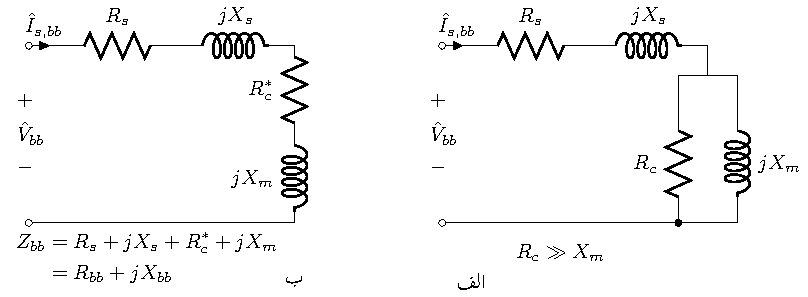
\includegraphics{figInductionUnloaded}
\caption{بے بوجھ امالی موٹر کا معائنہ۔}
\label{شکل_امالی_بے_بار_معائنہ}
\end{figure}

شکل \حوالہ{شکل_امالی_بے_بار_معائنہ}-ب سے ہم لکھ سکتے ہیں۔
\begin{gather}
\begin{aligned}
R_{bb}&=\frac{p_{bb}}{3 I_{s,bb}^2}\\
Z_{bb}&=\frac{V_{bb}}{I_{s,bb}}\\
X_{bb}&=\sqrt{\abs{Z_{bb}}^2-R_{bb}^2}\\
X_{bb}&=X_s+X_m
\end{aligned}
\end{gather}
یوں اس معائنہ سے موٹر کی بے بوجھ متعاملیت \عددیء{X_{bb}} حاصل ہوتی ہے۔اگر کسی طرح ساکن لچھے کی متعاملیت \عددیء{X_s} معلوم ہو تب اس مساوات سے \عددیء{X_m} حاصل کی جا سکتی ہے۔اگلے معائنہ میں ہم \عددیء{X_s}  کا اندازہ لگا سکیں گے۔

\جزوحصہ{جامد موٹر کا معائنہ}
یہ معائنہ ٹرانسفارمر کے کسرِ دور معائنہ کی طرح ہے۔ اس میں مشین کے رِستا امالوں کی معلومات حاصل ہوتی ہے۔البتہ امالی موٹر کا مسئلہ ذرا زیادہ پیچیدہ ہے۔امالی موٹر کی رِستا امالہ گھومتے لچھوں میں برقی تعدد اور قالب کے سیراب ہونے پر منحصر ہوتے ہیں۔

 اس معائنہ میں امالی موٹر کے گھومتے حصے کو حرکت کرنے سے زبردستی روک دیا جاتا ہے جبکہ ساکن لچھوں پر بیرونی برقی دباؤ \عددیء{V_{rk}} لاگو کر کے برقی طاقت \عددیء{p_{rk}} اور ساکن لچھوں کی برقی رو \عددیء{I_{s,rk}} ناپی جاتی ہیں۔ اصولی طور پر یہ معائنہ اُن حالات کو مدِ نظر رکھ کر کیا جاتا ہے جن پر موٹر کی معلومات درکار ہوں۔

جس لمحہ ایک موٹر کو ساکن حالت سے چالو کیا جائے اس لمحہ موٹر کی سرک ایک کے برابر ہوتی ہے اور اس کے گھومتے لچھوں میں عام تعدد \عددیء{ f_e}  کی برقی رو\حاشیہد{اس لمحہ کے برقی رو کو چھوٹی لکھائی میں وقت صفر سے منسلک کیا گیا ہے یعنی  \عددیء{t=0}} \عددیء{I_{t=0}} ہوتی ہے، لہٰذا اگر اس لمحہ کے نتائج درکار ہوں تو موٹر کے ساکن لچھوں پر عام تعدد یعنی \عددیء{f_e}  کی اتنی برقی دباؤ لاگو کی جائے گی جتنی سے اس کے گھومتے لچھوں میں برقی رو \عددیء{I_{t=0}} ہو۔ اسی طرح اگر عام چالو حالت میں بوجھ بردار موٹر کے نتائج درکار ہوں جب موٹر کی سرک \عددیء{s} اور اس کے گھومتے لچھوں میں برقی رو\حاشیہد{زیر نوشت  میں \عددیء{t \to \infty} اس بات کو ظاہر کرتی ہے کہ موٹر کافی دیر سے چالو ہے اور یہ ایک برقرار رفتار تک پہنچ گئی ہے۔} \عددیء{I_{t\to \infty}} ہوتی ہے تو معائنہ میں \عددیء{s f_e} تعدد کی برقی دباؤ استعمال کی جائے گی اور اس کی مقدار اتنی رکھی جائے گی جتنی سے گھومتے لچھوں میں \عددیء{I_{t\to \infty}} برقی رو وجود میں آئے۔تقریباً  \عددیء{\SI{20}{\kilo \volt \ampere}} سے چھوٹی موٹروں میں برقی تعدد کے اثرات قابلِ نظر انداز ہوتے ہیں لہٰذا ان کا معائنہ \عددیء{f_e} تعدد کی برقی دباؤ پر ہی کیا جاتا ہے۔

یہاں صفحہ \حوالہصفحہ{شکل_امالی_مشین_کا_مکمل_مساوی_دور} پر دکھائے شکل \حوالہ{شکل_امالی_مشین_کا_مکمل_مساوی_دور}  کو رکے موٹر کے معائنہ کی نقطہ نظر سے دوبارہ بناتے ہیں۔رکے موٹر کی سرک ایک کے برابر ہوتی ہے۔مزید یہ کہ اس معائنہ میں لاگو برقی دباؤ عام چالو موٹر پر لاگو برقی دباؤ سے خاصی کم ہوتی ہے۔اتنی کم لاگو برقی دباؤ پر قالبی ضیاع کو نظرانداز کیا جا سکتا ہے۔شکل میں  \عددیء{R_c} کو کھلے دور کرنا قالبی ضیاع کو نظرانداز کرنے کے مترادف ہے۔ایسا کرنے سے شکل \حوالہ{شکل_امالی_رکے_موٹر_معائنہ}-الف ملتا ہے۔چونکہ \عددیء{s=1} ہے لہٰذا اس شکل میں \عددیء{\tfrac{R_r'}{s}}  کو \عددیء{R_r'} لیا گیا ہے۔
\begin{figure}
\centering
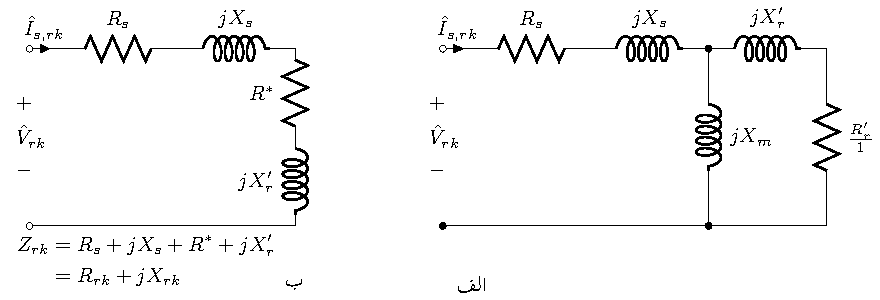
\includegraphics[width=\linewidth]{figInductionBlockedRotorTest}
\caption{رکے امالی موٹر کا معائنہ۔}
\label{شکل_امالی_رکے_موٹر_معائنہ}
\end{figure}

شکل  \حوالہ{شکل_امالی_رکے_موٹر_معائنہ}-الف میں \عددیء{j X_m}  اور \عددیء{(R_r'+j X_r')} متوازی جڑے ہیں۔ ان کا مساوی سلسلہ وار دور شکل \حوالہ{شکل_امالی_رکے_موٹر_معائنہ}-ب میں دکھایا گیا ہے۔اس متوازی دور کی مزاحمت \عددیء{Z_m} سے سلسلہ وار مزاحمت \عددیء{Z_s}  یوں حاصل ہوتی ہے۔
\begin{gather}
\begin{aligned}
Z_m&=\frac{j X_m (R_r'+j X_r')}{R_r'+j(X_m+X_r')}\\
&=\left( \frac{j X_m R_r' -X_m X_r'}{R_r'+j(X_m+X_r')} \right) \left( \frac{R_r'-j(X_m+X_r')}{R_r'-j(X_m+X_r')}\right)\\
&=\frac{jX_m R_r'^2+X_m R_r'(X_m+X_r')-X_m X_r' R_r' +j X_m X_r'(X_m+X_r')}{R_r'^2+(X_m+X_r')^2}\\
&=\frac{X_m^2 R_r'}{R_r'^2+(X_m+X_r')^2}+\frac{j(X_m R_r'^2+X_m^2 X_r'+X_m X_r'^2)}{R_r'^2+(X_m+X_r')^2}\\
&=R_s^*+j X_s^* =Z_s
\end{aligned}
\end{gather}
اگر ان مساوات میں \عددیء{X_m \gg R_r'} اور \عددیء{X_m \gg X_r'}  لیا جائے تو حاصل ہوتا ہے۔
\begin{align}\label{مساوات_امالی_تقریبا_مزاحمت}
R_s^*& \approx R_r' \left(\frac{X_m}{X_m+X_r'} \right)^2 \\
X_s^*&= \approx  \frac{X_m R_r'^2}{X_m^2}+\frac{X_m^2 X_r'}{X_m^2}+\frac{X_m X_r'^2}{X_m^2} \approx X_r'
\end{align}
اس معائنہ میں ناپے مقداروں اور شکل \حوالہ{شکل_امالی_رکے_موٹر_معائنہ}-ب سے
\begin{gather}
\begin{aligned}
Z_{rk} &=\frac{V_{rk}}{I_{s,rk}}\\
R_{rk}&=\frac{p_{rk}}{3 I_{s,rk}^2}\\
X_{rk}&=\sqrt{\abs{Z_{rk}}^2-R_{rk}^2}
\end{aligned}
\end{gather}
حاصل ہوتے ہیں۔ اس مساوات کے پہلے جزو میں ناپے برقی دباؤ اور برقی رو سے رکاوٹ حاصل کی گئی ہے، اس کے دوسرے جزو سے مزاحمت اور تیسرے میں متعاملیت۔

اب شکل \حوالہ{شکل_امالی_رکے_موٹر_معائنہ}-ب سے واضح ہے کہ 
\begin{align}
X_{rk}=X_s+X_r'
\end{align}
امالی مشین مختلف خصوصیات کو مد نظر رکھ کر بنائے جاتے ہیں۔عام  آدمی کے آسانی کے لئے ایسے مشینوں کی درجہ بندی کی جاتی ہے۔جدول \حوالہ{جدول_امالی_امالہ_کا_تقسیم} میں پنجرا نما امالی موٹر کے مختلف اقسام \عددیء{A,B,C,D} اور ایسی مشین جن کا گھمتا حصہ لچھے پر مشتمل ہو،  کے رِستا متعاملیت  \عددیء{X_{rk}} کو ساکن اور گھومتے لچھوں میں  تقسیم کرنا دکھایا گیا ہے۔اس جدول کے مطابق، گھومتے لچھے والی مشین میں ساکن اور گھومتے متعاملیت برابر ہوتے ہیں۔
\begin{table}
\begin{tabular}{r r c c}
گھومتا حصہ &خاصیت& \عددیء{X_s} & \عددیء{X_r'}\\
\hline\\
لپٹا ہوا & کارکردگی گھومتے حصے کی مزاحمت پر منحصر&\عددیء{0.5 X_{rk}} & \عددیء{0.5 X_{rk}} \\
بناوٹ \عددیء{A} &عام ابتدائی قوت گردشہ، عام ابتدائی رو& \عددیء{0.5 X_{rk}} & \عددیء{0.5 X_{rk}} \\
بناوٹ \عددیء{B} & عام ابتدائی قوت گردشہ، کم ابتدائی رو&\عددیء{0.4 X_{rk}} & \عددیء{0.6 X_{rk}} \\
بناوٹ \عددیء{C} &زیادہ ابتدائی قوت گردشہ، کم ابتدائی رو &\عددیء{0.3 X_{rk}} & \عددیء{0.7 X_{rk}} \\
بناوٹ \عددیء{D} &زیادہ ابتدائی قوت گردشہ، زیادہ سرک &\عددیء{0.5 X_{rk}} & \عددیء{0.5 X_{rk}} 
\end{tabular}
\caption{متعاملیت کی ساکن اور گھومتے حصوں میں تقسیم۔}
\label{جدول_امالی_امالہ_کا_تقسیم}
\end{table}
%
اسی طرح شکل  \حوالہ{شکل_امالی_رکے_موٹر_معائنہ}-ب سے واضح ہے کہ \عددیء{R_{rk}=R^*+R_s} لہٰذا اگر ساکن لچھے کی مزاحمت \عددیء{R_s}  براہِ راست مزاحمت ناپنے کے آلہ یعنی \اصطلاح{اوہم میٹر}\فرہنگ{اوہم میٹر}\حاشیہب{Ohm meter} سے ناپی جائے تو
\begin{align}
R^*=R_{rk}-R_s
\end{align}
ہو گا اور اب \عددیء{R_r'} کو مساوات \حوالہ{مساوات_امالی_تقریبا_مزاحمت}  سے حاصل کیا جا سکتا ہے جہاں \عددیء{X_m} بے بوجھ امالی موٹر کے معائنہ میں حاصل کی جاتی ہے۔

اوہم میٹر کی مدد سے ساکن لچھے کی مزاحمت ناپتے وقت یہ جاننا ضروری ہے کہ موٹر ستارہ یا تکونی جڑی ہے۔شکل \حوالہ{شکل_امالی_ساکن_مزاحمت_کا_حصول}  میں لچھے کو دونوں طرح جڑا دکھایا گیا ہے۔ اگر یک مرحلہ مزاحمت \عددیء{R_s}  ہو تو ستارہ جڑی موٹر میں اوہم میٹر  \عددیء{2 R_s} مزاحمت دے گی جبکہ تکونی جڑی موٹر کے لئے یہ \عددیء{\tfrac{2}{3} R_s} مزاحمت دے گی۔
\begin{figure}
\centering
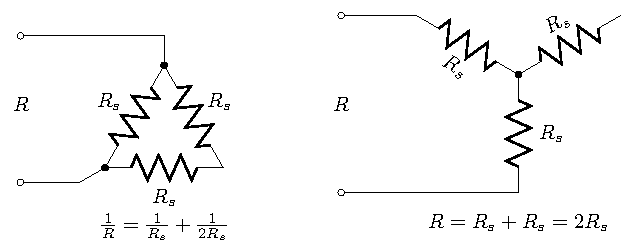
\includegraphics{figInductionStarDeltaStator}
\caption{ستارہ اور تکونی جڑی موٹروں کی ساکن لچھوں کی مزاحمت کا اوہم میٹر کی مدد سے حصول۔}
\label{شکل_امالی_ساکن_مزاحمت_کا_حصول}
\end{figure}

\ابتدا{مثال}
ستارہ جڑی چار قطب پچاس ہرٹز اور \عددیء{415} وولٹ پر چلنے والی موٹر کے معائنہ کئے جاتے ہیں۔ موٹر کی بناوٹ درجہ بندی \عددیء{A}  کے مطابق ہے۔اوہم میٹر کسی بھی دو برقی سروں کے مابین \عددیء{0.55} اوہم جواب دیتا ہے۔بے بوجھ معائنہ \عددیء{\SI{50}{\hertz}} اور \عددیء{\SI{415}{\volt}} پر کرتے ہوئے برقی رو \عددیء{\SI{4.1}{\ampere}} اور طاقت کا ضیاع \عددیء{\SI{906}{\watt}} ناپے جاتے ہیں۔جامد موٹر معائنہ  \عددیء{\SI{15}{\hertz}} اور \عددیء{\SI{50}{\volt}} پر کرتے ہوئے برقی رو \عددیء{\SI{13.91}{\ampere}} اور طاقت کا ضیاع \عددیء{\SI{850}{\watt}} ناپے جاتے ہیں۔اس موٹر کی مساوی برقی دور بنائیں اور پانچ فی صد سرک پر اس کی اندرونی میکانی طاقت حاصل کریں۔

حل:
	اوہم میٹر کے جواب سے  ستارہ جڑی موٹر کے ساکن لچھے کی مزاحمت \عددیء{R_s=\tfrac{0.55}{2}=\SI{0.275}{\ohm}} حاصل ہوتی ہے۔بے بوجھ معائنہ میں یک مرحلہ برقی دباؤ \عددیء{\tfrac{415}{\sqrt{3}}=\SI{239.6}{\volt}} ہے جس سے
\begin{align*}
R_{bb} &=\frac{906}{3 \times 4.1^2}=\SI{17.965}{\ohm}\\
\abs{Z_B}&=\frac{239.6}{4.1}=\SI{58.439}{\ohm}\\
X_{bb}&=\sqrt{58.439^2-17.965^2}=\SI{55.609}{\ohm}=X_s+X_m
\end{align*}
لہٰذا  رکے موٹر معائنہ کے نتائج سے \عددیء{X_s} حاصل کرنے کے بعد \عددیء{X_m} حاصل ہو جائے گی۔

ساکن لچھے کی مزاحمت میں اس برقی رو پر کُل
\begin{align*}
3 I_{bb}^2 R_s=3 \times 4.1^2 \times  0.275=\SI{13.87}{\watt}
\end{align*}
برقی طاقت کا ضیاع ہو گا لہٰذا رگڑ اور دیگر طاقت کا ضیاع \عددیء{906-13.86=892} واٹ ہو گا۔

رکے موٹر کے معائنہ میں یک مرحلہ برقی دباؤ \عددیء{\tfrac{50}{\sqrt{3}}=28.9} وولٹ ہیں یوں اس معائنہ سے
\begin{align*}
R_{rk}&=\frac{850}{3 \times 13.91^2}=\SI{1.464}{\ohm}\\
\abs{Z_{rk}}&=\frac{28.9}{13.91}=\SI{2.07}{\ohm}\\
X_{rk, 15}&=\sqrt{2.07^2-1.464^2}=\SI{1.46}{\ohm}
\end{align*}
حاصل ہوتے ہیں۔ اس معائنہ میں برقی تعدد \عددیء{15} ہرٹز تھی لہٰذا \عددیء{50} ہرٹز پر متعاملیت
\begin{align*}
X_{rk,50}=\frac{50}{15} \times X_{rk,15} \approx \SI{4.9}{\ohm}
\end{align*}
ہے۔درجہ بندی \عددیء{A} کی امالی موٹر کے لئے یہ متعاملت ساکن اور گھومتے لچھے میں یکساں تقسیم ہوتی ہے لہٰذا
\begin{align*}
X_s=X_r'=\frac{4.9}{2}=\SI{2.45}{\ohm}
\end{align*}
یوں
\begin{align*}
X_m=X_{bb}-X_s=55.609-2.45=\SI{53}{\ohm}
\end{align*}
چونکہ  \عددیء{R_s=0.275} اوہم ہے  لہٰذا
\begin{align*}
R_r'=R_{rk}-R_s=1.464-0.275=\SI{1.189}{\ohm}
\end{align*}
ہو گا۔یہ مساوی برقی دور شکل \حوالہ{شکل_امالی_موٹر_مثال_کا_دور} میں دکھایا گیا ہے۔
\begin{figure}
\centering
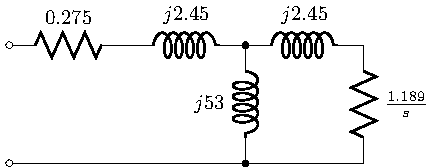
\includegraphics{figInductionMachineEquivalentCircuitExample}
\caption{امالی موٹر کی مساوی برقی دور۔}
\label{شکل_امالی_موٹر_مثال_کا_دور}
\end{figure}

پانچ فی صد سرک پر اندرونی میکانی طاقت کی خاطر بائیں جانب کا تھوِنن مساوی دور استعمال کرتے ہوئے 
\begin{align*}
V_t&=229 \phase{0.2833 \degree}\\
Z_t&=0.251+j2.343\\
\abs{\hat{I}_r'}&=\SI{11.8}{\ampere}\\
p_m&=\frac{3 \times 11.8^2 \times 0.974 \times (1-0.05)}{0.05}=\SI{7730}{\watt}
\end{align*}
\انتہا{مثال}
